%You can delete all the comments after you have finished your document
%this sets up the defaults for the documents, 12pt font and A4 size. The article type sets this up as such as opposed to letter or memo.

%for the finer points LaTeX see https://en.wikibooks.org/wiki/LaTeX or http://tex.stackexchange.com/

\documentclass[12pt,a4paper]{article}
\usepackage{titlesec} %these are how we import packages, one helps set up footers and title layout
\usepackage{fancyhdr}

% !TEX TS-program = pdflatex
% !TEX encoding = UTF-8 Unicode
\usepackage[utf8]{inputenc} % set input encoding (not needed with XeLaTeX)

\usepackage{graphicx} % support the \includegraphics command and options
\graphicspath{ {images/} } % tells LATEX that the images are kept in a folder named images under the current directory.

% \usepackage[parfill]{parskip} % Activate to begin paragraphs with an empty line rather than an indent

%%% PACKAGES
\usepackage{booktabs} % for much better looking tables
\usepackage{array} % for better arrays (eg matrices) in maths
\usepackage{paralist} % very flexible & customisable lists (eg. enumerate/itemize, etc.)
\usepackage{verbatim} % adds environment for commenting out blocks of text & for better verbatim
\usepackage{subfig} % make it possible to include more than one captioned figure/table in a single float
\usepackage[toc,page]{appendix}
% These packages are all incorporated in the memoir class to one degree or another...
\usepackage{pdfpages}
% Testing to see how IPO will look as I use this and use it as a pdf
\usepackage{csquotes}
%" facing the wrong way so trying to rectify that

\usepackage[breaklinks = true]{hyperref}
\hypersetup
{
	colorlinks=false, %set true if you want colored links
	linktoc=all,     %set to all if you want both sections and subsections linked
}
%\usepackage[hyphenbreaks]{breakurl}
\usepackage[anythingbreaks]{breakurl}
\usepackage{gensymb}
\usepackage[round]{natbib}

\usepackage{tabu}

%header and footer settings
\pagestyle{fancyplain}
\fancyhf{}
\renewcommand{\headrulewidth}{0.5pt}
\renewcommand{\footrulewidth}{0.5pt}
\setlength{\headheight}{15pt}
\fancyhead[L]{Ryan O'Flaherty - 40168766}
\fancyhead[R]{SOC10101 Honours Project}
\fancyfoot[L]{}
\fancyfoot[C]{\thepage}

%set better section layout
\makeatletter
\renewcommand\subsection{\@startsection {subsection}{1}{2mm} % name, level, indent
                               {3pt plus 2pt minus 1pt} % before skip
                               {3pt plus 0pt} % after skip
                               {\normalfont\bfseries}}
\makeatother
\makeatletter
\renewcommand\section{\@startsection {section}{1}{0mm} % name, level, indent
                               {4pt plus 2pt minus 1pt} % before skip
                               {4pt plus 0pt} % after skip
                               {\bfseries}}
\makeatother


%this starts the document
\begin{document}

%you can import other documents into your main one, these layout the Title and Declarations on its own page.
%you might need to change these to \ if your on Microsoft Windows.
\newcommand{\HRule}{\rule{\linewidth}{0.5mm}}

\begin{titlepage}
	\begin{center}

	\HRule \\[0.4cm]
    	{\Large \bfseries Evolution of Neural Network Controllers\\for Gameplay Behaviours\par}
	\vspace{0.2cm}
	\HRule \\[1.5cm] 

	
    	\vspace{3cm}
	\begin{minipage}{0.4\textwidth}
	\begin{center} \large
        \emph{}\\
        	Ryan O'Flaherty 40168766
				
   	 \end{center}
    	\end{minipage}
	
	\vspace{2cm}
    	\begin{minipage}{1\textwidth}
    	\begin{center} \large
        
		Submitted in partial fulfilment of \\
		the requirements of Edinburgh Napier University \\
		for the Degree of \\
        	BSc (Hons) Games Development
    	\end{center}
    	\end{minipage}

    	\vfill

    	% Bottom of the page
	\begin{minipage}{1\textwidth}
    	\begin{center} \large
		School of Computing
    	\end{center}
    	\end{minipage}
	
	\vspace{1cm}
    	{\large \today}


	\end{center}
\end{titlepage}
%{\large Submitted in partial fulfilment of the requirements of Edinburgh Napier University for the Degree of }
\clearpage
\section*{Authorship Declaration}
\vspace{0.5cm}
\begin{flushleft}
I, Ryan O'Flaherty, confirm that this dissertation and the work presented in it are my own achievement.\newline

Where I have consulted the published work of others this is always clearly attributed;\newline

Where I have quoted from the work of others the source is always given. With the exception of such quotations this dissertation is entirely my own work;\newline

I have acknowledged all main sources of help; \newline

If my research follows on from previous work or is part of a larger collaborative research project I have made clear exactly what was done by others and what I have contributed myself;\newline

I have read and understand the penalties associated with Academic Misconduct.\newline

I also confirm that I have obtained informed consent from all people I have involved in the work in this dissertation following the School's ethical guidelines.\newline
\end{flushleft}

\begin{flushleft} \large
\emph{Signed:} \\
\end{flushleft}

\vspace{.5cm}

\begin{flushleft} \large
\emph{Date:} \\
\end{flushleft}

\vspace{.5cm}

\begin{flushleft} \large
\emph{Matriculation no: }  \\
\end{flushleft}
\thispagestyle{empty}
\pagebreak
\clearpage
\section*{Data Protection Declaration}
\vspace{0.5cm}
\begin{flushleft}
Under the 1998 Data Protection Act, The University cannot disclose your grade to an unauthorised person. However, other students benefit from studying dissertations that have their grades attached. \newline

\vspace{0.5cm}

Please sign your name below one of the options below to state your preference.\newline
\vspace{0.5cm}

The University may make this dissertation, with indicative grade, available to others.\newline
\vspace{3cm}


The University may make this dissertation available to others, but the grade may not be disclosed.\newline
\vspace{3cm}


The University may not make this dissertation available to others.\newline
\end{flushleft}


\thispagestyle{empty}
\pagebreak

\pagenumbering{roman}
\setcounter{page}{1}

%LaTeX let you define the abstract separately so it wont get sucked into the main document.
\begin{abstract}
	Neural networks and evolutionary algorithms have been paired in game-related research and experimental projects in the field of artificial intelligence many times before, but similar papers are hard to come by when applied to card games.
	
	Recreating and using the card game Switch, an investigation into the effectiveness of a machine learning technique of this type in such an environment will take place.
	
\begin{center}
% fill the abstract in here
$\clubsuit$ \\

$ \diamondsuit$ \\ 

$ \heartsuit$ \\

$ \spadesuit$
\end{center}



\end{abstract}
\pagebreak

%\pagenumbering{arabic}
%\tableofcontents % is generated for you
%\pagenumbering{roman}
\newpage



\cleardoublepage
% Let's change \thepage so it prints one less than
% the real page number; \pagenumbering{arabic}
% will redefine it to the right meaning afterwards.
\renewcommand\thepage{\romannumeral\numexpr\value{page}\relax}

\tableofcontents

\cleardoublepage

\listoftables
%generated in same way as figures
\newpage

\listoffigures
%you may have captions such as equations, listings etc they should all appear as required
%these are done for you as long as you use \begin{figure}[placement settings] .. bla bla ... \end{figure}
\newpage

\section*{Acknowledgements}
The Games Development course has been journey of personal development in addition to gaining a higher education by obtaining and improving existing skills. I would like to thank my family and friends for ensuring that I remained as positive as possible throughout not only this project but my degree as a whole. I am particularly thankful to those who encouraged me to further my education in the first place.\\

%It has been the proverbial roller-coaster ride with several highs, lows, moments of complete disorientation, and a feeling of wishing you could do it all over again. The last four years have gone by in the blink of an eye, but have provided experiences and created friendships that will remain far beyond graduation.\\

%I would like to thank my friends and family for ensuring that I remained positive and motivated along the way, and for their participation in the testing phases. All of the support, assistance and feedback has been invaluable to both myself and the project as a whole. \\

I am also hugely appreciative of my project supervisor, Dr Simon Powers. Simon has provided me with excellent support and guidance throughout the process and for that I am eternally grateful. %Toy Story reference that probably sounds daft 

%I would like to thank Calum and Steven for abstaining from Fortnite duties on the night of 24/03/18 as not having my squaddies meant actually fixing this fucking thing.

%Also, cheers to my supervisor, I suppose. 

\newpage
\setcounter{page}{1}
\pagenumbering{arabic}

\section{Introduction}
Card games appear to be an unexplored area in relation to neuro-evolution, and this project intends change that. This chapter outlines the project plan for how that will be achieved. \\

\subsection{Aims and Objectives}

The goal of this project is to develop a card game, and incorporate an artificially intelligent autonomous player. The underlying purpose of the project is to research and demonstrate the effectiveness of artificial neural networks and evolutionary algorithms in a game of this type.  \\

In order to achieve this goal, smaller objectives must be reached. These include researching and learning about neural networks and evolutionary algorithms, building a card game from scratch, and then gathering data from an extensive testing regime. This data must then be critically evaluated and discussed. \\

\subsection{Scope}
The game will be constructed for two to four players - human or otherwise. An increased number of players may break the game due to running out of cards. \\

\subsection{Constraints}
The project begins as a first endeavour into researching and working with artificial intelligence techniques. As a result, this project will not only involve the development of an intricate game system, and gathering and evaluating experimental results, but a lot of learning will also need to take place. \\

\subsection{Sources of Information} 
Sixteen years prior to this project, researchers at The University of Texas at Austin published a paper in which they detailed the development of their innovative neural network evolution library\citep{NEAT} entitled, \enquote{NeuroEvolution of Augmenting Topologies,} or \enquote{NEAT} in abbreviated form. The library has been converted to several programming languages over the years; However, this project will stick with the original C++ version. The NEAT library will be discussed in depth in the Methodology section of this dissertation.

The documentation file in Appendix G will be used to aid work with the NEAT library.\\

%This project will be built in C++, and will need to be compiled to a minimum of C++11 standard due to the use of shared pointers.\\

The graphical element of the project will be developed with Simple and Fast Multimedia Library (SFML) imported. SFML \enquote{provides a simple interface to the various components of your PC, to ease the development of games and multimedia applications\citep{SFML}.}\\


\subsection{Dissertation Structure}
The current chapter provides an introduction to the project, explaining the ambitions and rationale. Chapter 2 provides a background to the field of artificial intelligence with respect to games development. This is followed by a literature review, discussing previous and current projects with similarities to this topic. The rules of the Switch card game are briefly explained in Chapter 4, before Chapter 5 explains the technicalities of the development phase. Results are then discussed, and Chapter 7 evaluates the project as a whole. A summary is provided in the final chapter. \\

 \subsection{Overview Of Project Content and Milestones}
Milestones and objectives for the project are as follows: 
\subsubsection{Research}
Neural networks and evolutionary algorithms research are necessary to aid with the project development and to make up for current lack of knowledge.

\subsubsection{Game Foundation}
A short-term goal of the project is to create a bare-bones version of the card game without any artificial intelligence. This has to be created as it is the foundation on which the rest of the project will reside, and as such it needs to be rigorously tested to ensure that the rules of the game have been correctly implemented without any bugs. That way, any future problems will be related to the artificial intelligence itself.

\subsubsection{Implementation of Artificial Intelligence}
Most likely the phase of greatest difficulty and complexity, the implementation of artificial neural networks and evolutionary algorithms is expected to be a largely time consuming task. 

This will be where the game will transition from a hard-coded, bare-bones implementation to something of more interest. Once this has been successfully set up, we can begin testing and tweaking it to analyse the varying results.

\subsubsection{Experiments and Testing}
A large amount of games will be required to allow the evolution process to grow into something that performs to a decent level in our game. This will mean the game will have to be played multiple times, and so it will be beneficial to get other people to play-test the game too. 

Each time tweaks are made in our algorithm, the game will need to be thoroughly re-tested, with the results of these tests being accurately documented to provide a solid basis for the next stage of tweaking. 

The aim is to have a very large set of data to analyse and draw conclusions from in the latter stages of the project. 

\subsubsection{Evalution and Conclusion}
The aforementioned dataset will be used extensively to deeply examine the performance of each machine learning techniques implemented throughout the experimental stage of the project, with regards to both our hard-coded solutions and the results of other attempted solutions. 

\newpage
\section{Background}
\subsection{Introduction}
The following section of this dissertation will go on to discuss the history of artificial intelligence within the context of video games, before going on to explain neural networks, evolutionary algorithms, and the NeuroEvolution of Augmenting Topologies (NEAT) library.\\

\subsection{History of AI in Games}
Video games have been a popular area of interest for artificial intelligence developers and researchers for many decades. 

Over several tens of years, a large amount of research and development has been done in an attempt to perfect chess-playing artificial intelligence agents\citep{L2PChess}, and work has more recently been put in to do the same with the game of Go.  

In March of 2016, the goal of getting such an agent to compete and win at the highest level was reached when AlphaGo, a program engineered by Google, managed to overcome the Go world champion human player, Lee Sedol\citep{ABriefHistoryOfGameAI}. This was then reported as a major breakthrough for the artificial intelligence field. 

With Go, developers are unable to use brute force approaches due to the vastly complex nature of the game\citep{13}. In other words, the complexity of Go means that a strategy cannot be hard-coded to play the game, and things like search trees are not applicable either. AlphaGo's solution to this was the implementation of a neural network to learn and play the game, taking into consideration millions of game states from previous games involving human expert players. 

This would theoretically result in AlphaGo performing at a similar level to that of the human players it learned from. To go above and beyond that level, and to be able to beat a champion like Sedol, AlphaGo was then put up against itself, consequently improving with every game it played\citep{13}. It can be said that in this phase, AlphaGo literally taught itself. 

In terms of Chess, a machine managed to win against a human of World Champion status named Gerry Kasparov in the late 1990s\citep{14}. That machine was Deep Blue. In actual fact, it was the second version of IBM's Deep Blue. The first Deep Blue lost to the same opponent a year prior to its successor's achievement in 1997\citep{14}. That success came in the form of two wins, a loss, and three draws\citep{15}, over the course of several days. However, IBM did not use artificial intelligence with Deep Blue, relying instead on computational power and a less complex search and evaluation function\citep{16}. \\

\subsection{What is a Neural Network?}
Artificial neural networks, commonly referred to simply as neural networks, are a rough representation of the human brain. Human brains can be thought of as highly complex and non-linear systems for processing information in parallel\citep{NeuralNetworksAComprehensiveFoundation}. 

To emulate this, neural networks are built using a series of layers of network nodes. These nodes are used to represent neurons in the brain. The first is an input layer, followed by two or three hidden layers before a final output layer of nodes\citep{ArtificialNeuralNetwork}. The connection between these nodes is representative of axons in the brain. 

In an artificial neural network, the input and output layers take data in and produce results respectively, with the processing of said data being done within the hidden layers - but how does it work? 

\subsubsection{Perceptrons}
One type of artificial neuron (or node) is known as a \enquote{perceptron.} Each perceptron receives several inputs and uses them to produce one binary output\citep{NeuralNetworksAndDeepLearning}.  

\begin{figure}[h]
	\centering
	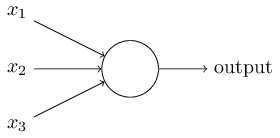
\includegraphics{Perceptron.png}
	\caption{A Single Perceptron}
	\centering{\citep{NeuralNetworksAndDeepLearning}}
\end{figure}

Frank Rosenblatt, the scientist who developed the perceptron in the 1950s and 1960s, devised a rule for computing the output from these neurons. Using what he called \enquote{weights,} the importance of each input is assessed and expressed. Each input has a weight assigned to it, and the resultant output from these inputs - either a 1 or 0 - is dependent on whether or not some threshold value is less than or greater than the sum of the weights from all of the inputs to that particular perceptron. Therefore, if the weighted sum is less than or equal to the threshold value, the output is a 0; Otherwise, a 1\citep{NeuralNetworksAndDeepLearning}. Both the threshold value and the input weights are real numbers. These can be tweaked to alter the decisions made by a neural network. 

\subsubsection{Sigmoid Neurons}

Sigmoid neurons are akin to perceptrons, however, they are modified in such a way that marginal alterations in their weights and bias cause only a small change to their output\citep{NeuralNetworksAndDeepLearning}. This crucial difference is what affords a network consisting of sigmoid neurons the ability to learn.

The inputs to a sigmoid neuron also differ from those of perceptrons. Rather than being binary (1 or 0), these inputs are any number \textit{between} 1 and 0. %probably pointless italics
Much like with perceptrons, these sigmoid neuron inputs are weighted, with an overall bias included. 

The shape of a plotted sigmoid function ($\sigma$) can be seen in Figure 2. 

\begin{figure}[h]
	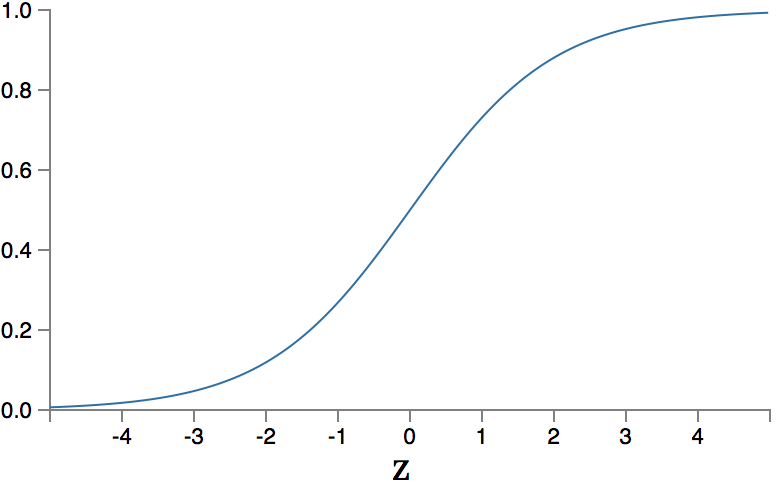
\includegraphics[width=\textwidth, height=5cm]{SigmoidFunction.png}
	\caption{Sigmoid Function} \centering{\citep{NeuralNetworksAndDeepLearning}}
\end{figure}

To give sigmoid neurons the smoothness required for a non-linear activation function, the following logistic function defining sigmoidal non-linearity is used:
\begin{eqnarray}
y_j = \frac{1}{1+exp(-v_j)}
\end{eqnarray}

\begin{center}
	\citep[Chapter 4, page 179] {NeuralNetworksAComprehensiveFoundation}
\end{center}

This calculates the output from our neuron \textit{{$y_j$}}, with \textit{j} being the neuron itself, and \textit{$v_j$} representing the sum of all inputs (with weighting applied) plus the bias\citep{NeuralNetworksAComprehensiveFoundation}.

Input weights can be calculated via the dot product. Thus, using \textit{w}, \textit{x} and \textit{b} as symbols for weights, inputs and bias, we can represent $v_j$ as 
\begin{eqnarray}
(w \cdot x+b).
\end{eqnarray}

\begin{center}
	\citep{NeuralNetworksAndDeepLearning}
\end{center}

Therefore, extending the output calculation gives us
\begin{eqnarray} 
%y_j = \frac{1}{1+\exp(-\sum_j w_j x_j-b)}.\\\\
y_j = \frac{1}{1+\exp(-\sum_j w_j \cdot x_j - b)}.
\end{eqnarray}


When $v_j$ is a large, positive number the sigmoid neuron output is approximately 1. On the other hand, the output is approximately 0 if $v_j$ is heavily negative. These outputs are similar to that of perceptrons. However, when $v_j$ is somewhere in between, the similarities cease. 

Even the smallest alterations to the weighting or bias can create small changes to the output from a sigmoid neuron, due to the smooth nature of the function\citep{NeuralNetworksAndDeepLearning}.\\

\subsection{Evolutionary Algorithms}
As the name might suggest, an evolutionary algorithm is one that evolves. It does so to encourage finding the most optimal solution to a problem. A vast amount of varying evolutionary algorithms exist, but at the core of them all is the same principal idea: \enquote{given a population of individuals the environmental pressure causes natural selection (survival of the fittest) and this causes a rise in the fitness of the population}\citep{IntroductionToEvolutionaryComputing}. As a result, the population adapts over time to its environment. 

What is the process of evolution? The generational cycle works as follows:

\subsubsection{Representation}
Step one when defining an evolutionary algorithm is to bridge the gap between the \enquote{real world} and the \enquote{evolutionary algorithm world}\citep{IntroductionToEvolutionaryComputing}. That is, to link what are known as phenotypes, to representative genotypes. 

%In order to use an evolutionary algorithm, possible solutions must be represented as what are known as chromosomes (or genotypes). 

\begin{itemize}
	\item Phenotype: A solution to a problem
	\item Genotype: Chromosome used to represent the solution to a problem
\end{itemize}

Representation refers to specifying which genotypes equate to each phenotype\citep{IntroductionToEvolutionaryComputing}. For example, if an integer is the solution to a problem, it is the phenotype, and a binary representation of that particular integer would be the genotype relating to that phenotype. 

A genotype (or chromosome) is made up of genes. Values are assigned to each gene, and may be referred to as alleles. These can be of any type, or even a mixture. Types include binary strings, integers, real values, permutations and symbols. So in the example above, each gene would be either a 1 or 0, combining to form the integer as an overall chromosome.

Sometimes it may not be quite so straightforward, and genotypes need to be explicitly mapped to phenotypes, as seen in Figure 3. 

\begin{figure}[h]
	\centering
	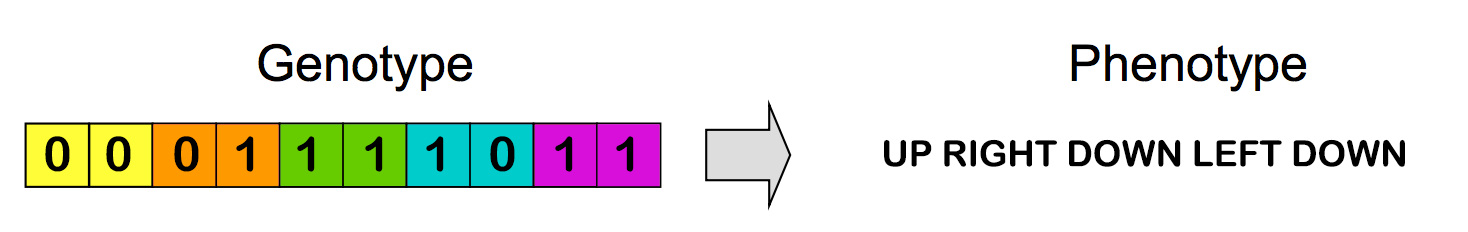
\includegraphics[width = \textwidth]{GenoToPheno.png}
	\caption{Genotype vs Phenotype}
\end{figure}


\subsubsection{Initialisation}
In the beginning, we start off with a population comprised completely of random chromosomes. This is likely to yield very poor results, however there is always a chance that some may be better. These individuals must then be evaluated.

\subsubsection{Fitness}
The fitness of an individual is what defines how fit for purpose it is. This measurement of quality will be defined differently for every algorithm, depending entirely on the context of problems it is being used to solve. In this project, the fitness will correlate to the amount of illegal moves the agent attempts to make, and how many times it is forced to increase its hand rather than decrease it. However, as the game of switch is largely down to luck, this will have to be taken into account to incorporate some form of leniency to fitness calculations.  

The role of an evaluation function (or fitness function) to encourage improvements by defining what an improvement is\citep{IntroductionToEvolutionaryComputing}. This lays the foundation for selection. 

\subsubsection{Selection}
The process of choosing individuals, based on their fitness, from the population to become parents to the next generation of individuals is called selection\citep{IntroductionToEvolutionaryComputing}. This is the driving force behind progressive evolution as it biases selection towards individuals of higher quality. 

\subsubsection{Crossover}
Sometimes referred to as recombination, crossover is an operation that merges genes from two parent genotypes together into one or two offspring genotypes\citep{IntroductionToEvolutionaryComputing}. 

Crossover can be defined in a few ways. There is one-point crossover, where a randomly chosen point along the length of a chromosome determines which genes are passed on from that particular genotype, and the rest will come from the other parent. This is demonstrated in Figure 4.

\begin{figure}[h]
	\centering
	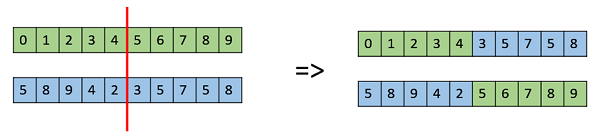
\includegraphics[width = \textwidth]{one_point_crossover.jpg}
	\caption{One-Point Crossover}
	\centering{\citep{crossover}}
\end{figure}

Next, n-point crossover is when more than one (n) point is chosen, and chromosomes can be split up in different ways, as seen in Figure 5. 

\begin{figure}[h]
	\centering
	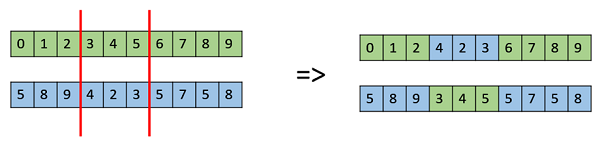
\includegraphics[width = \textwidth]{multi_point_crossover.jpg}
	\caption{N-Point Crossover}
	\centering{\citep{crossover}}
\end{figure}

%\newpage
Another type of crossover is called uniform. In this case, each gene of the offspring is randomly selected by deciding which of the two parents to inherit from. This is demonstrated in Figure 6.

\begin{figure}[h]
	\centering
	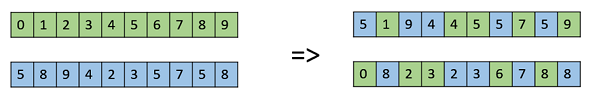
\includegraphics[width = \textwidth]{uniform_crossover.jpg}
	\caption{Uniform Crossover}
	\centering{\citep{crossover}}
\end{figure}


In the case of arithmetic crossover, an average of the two parent genes is calculated and used for the child gene. This is useful if the genes consist of real numbers. Figure 7 depicts this.

\begin{figure}[h]
	\centering
	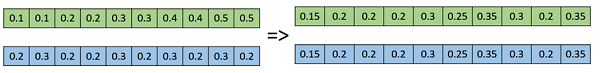
\includegraphics[width = \textwidth]{arith_crossover.png}
	\caption{Arithmetic Crossover}
	\centering{\citep{crossover}}
\end{figure}

All of the above techniques are used in binary and integer chromosome representations. Permutations cannot be recombined using any of these techniques, but are beyond the scope of this project. 

\subsubsection{Mutation}
When applied to a genotype, mutation returns a slightly mutated offspring\citep{IntroductionToEvolutionaryComputing}. It can create new genes in the population, which in turn diversifies the population. 

Like with crossover, there are different ways to perform mutation. In the case of binary chromosomes, we would allow each gene to 'flip' from a 1 to a 0 or vice versa, as demonstrated by Figure 8. Each gene has a probability of being mutated in this way, which will often be calculated as 1/\textit{n} with \textit{n} being representative of the chromosome length.


%Binary
\begin{figure}[h]
	\centering
	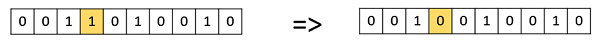
\includegraphics[width = \textwidth]{BinaryMutation.png}
	\caption{Binary Mutation}
	\centering{\citep{mutation}}
\end{figure}

\newpage
Integers are slightly different. The probability remains the same, but the difference is that a set of possible numbers, for example 0 to 9, is set up and when a gene is chosen for mutation, a number within that range is randomly generated and used in the offspring. 
 
Again, permutations work in a completely different way, but are not considered as part of this project. 

\subsubsection{Replacement}
This is the part where individuals are removed from the population to make way for a generation of new and hopefully improved genotypes. We could just remove the oldest genotype in the population, but this could be one with a high fitness! This can also be done randomly, but again there is a risk that we could be removing individuals of high quality. The other way is to determine which individuals to remove using the fitness. We could just get rid of the least fit genotypes, which could lead to the population improving very quickly, however it could also lead to premature convergence.\\

\newpage
\subsection{NeuroEvolution for Augmenting Topologies (NEAT)}
\enquote{NEAT is a method for evolving speciated neural networks of arbitrary structures and sizes. NEAT leverages the evolution of structure to make neuroevolution more efficient}\citep{NEAT}.

It is claimed to result in significantly faster learning than neuroevolution techniques using fixed network topologies.
 
 In NEAT, the mutation phase can alter network structures as well as connection weights\citep{EfficientEvolutionOfNeuralNetworkTopologies}. While connection weights are mutated in the same way as described in the previous section, network structure can be mutated in two ways:
 
 \begin{itemize}
 	\item Add Connection
 	\begin{itemize}
 		\item A new connection gene is added, linking two nodes that were not connected beforehand
 	\end{itemize}
 	\item Add Node
 	\begin{itemize}
 		\item A connection that already exists is split and the new node replaces the old connection. That previous connection is disabled and the genome gains two new connections. 
 	\end{itemize}
 \end{itemize}
 
 
 %SOME GOOD STUFF IN \citep{EvolvingARovingEyeForGo}

\newpage
\section{Literature Review}
Video games are a field that has been used as a catalyst for research and development in artificial intelligence due to the relatively risk-free nature of it when compared to other areas where AI might be used for quite some time now, but it was only recently that a program was able to beat a world class human player in the game of Go\citep{ABriefHistoryOfGameAI}. This is despite a huge amount of work and time being injected into developing these types of game-playing agents with the desired result of beating the best human players in the world at Chess, and more recently, Go. 

This project aims to create a digital version of the card game Switch. While playing, each competitor has no idea what cards are held by their opponent(s). They only know what cards they themselves hold, and what the most recently played card was. They will also know whose turn it is and what direction the play is going (if there are multiple remaining opponents). 

Solutions for Chess and Go might use search trees for decision making, however this requires knowing the full state of the game, including the location of every game piece on the board. This is what is known as \enquote{perfect information.} However, in card games such as Poker or Switch, there are unknowns such as the hands other players have or the value of cards that are face down. Therefore, we are faced with \textit{\enquote{imperfect information.}}\\

%The game can also be described as dynamic, as each player takes their turn in sequence. This sequence can also be reversed if a Jack card is played. 

%Making some notes here:\\

%I want to create the card game Switch - but the question is, how? \\

%From one he gave me:\\
%Chess and Go use search trees for decision making, however this requires knowing the full state of the game, including the location of every game piece on the board. This is what is known as 'perfect information.' However, in card games such as Poker or Switch, we do not know what hands other players have, nor do we know the value of cards that are face down. Therefore, we are faced with 'imperfect information.' \\

%This is where neural networks come in. \\\\\\\\

%Looking at dissertation he gave me
%Dynamic: Players take multiple turns taken in sequence
%Imperfect information

\subsection{AI for Playing Games}
When researching neural networks in relation to games, a stand-out is MarI/O. There is a video on YouTube showcasing its solution after 34 generations using NEAT. It is described on the page of that video as the following:\\

\textit{\enquote{MarI/O is a program made of neural networks and genetic algorithms that kicks butt at Super Mario World}}\citep{MarIO}.\\

\begin{figure}[h]
	\centering
	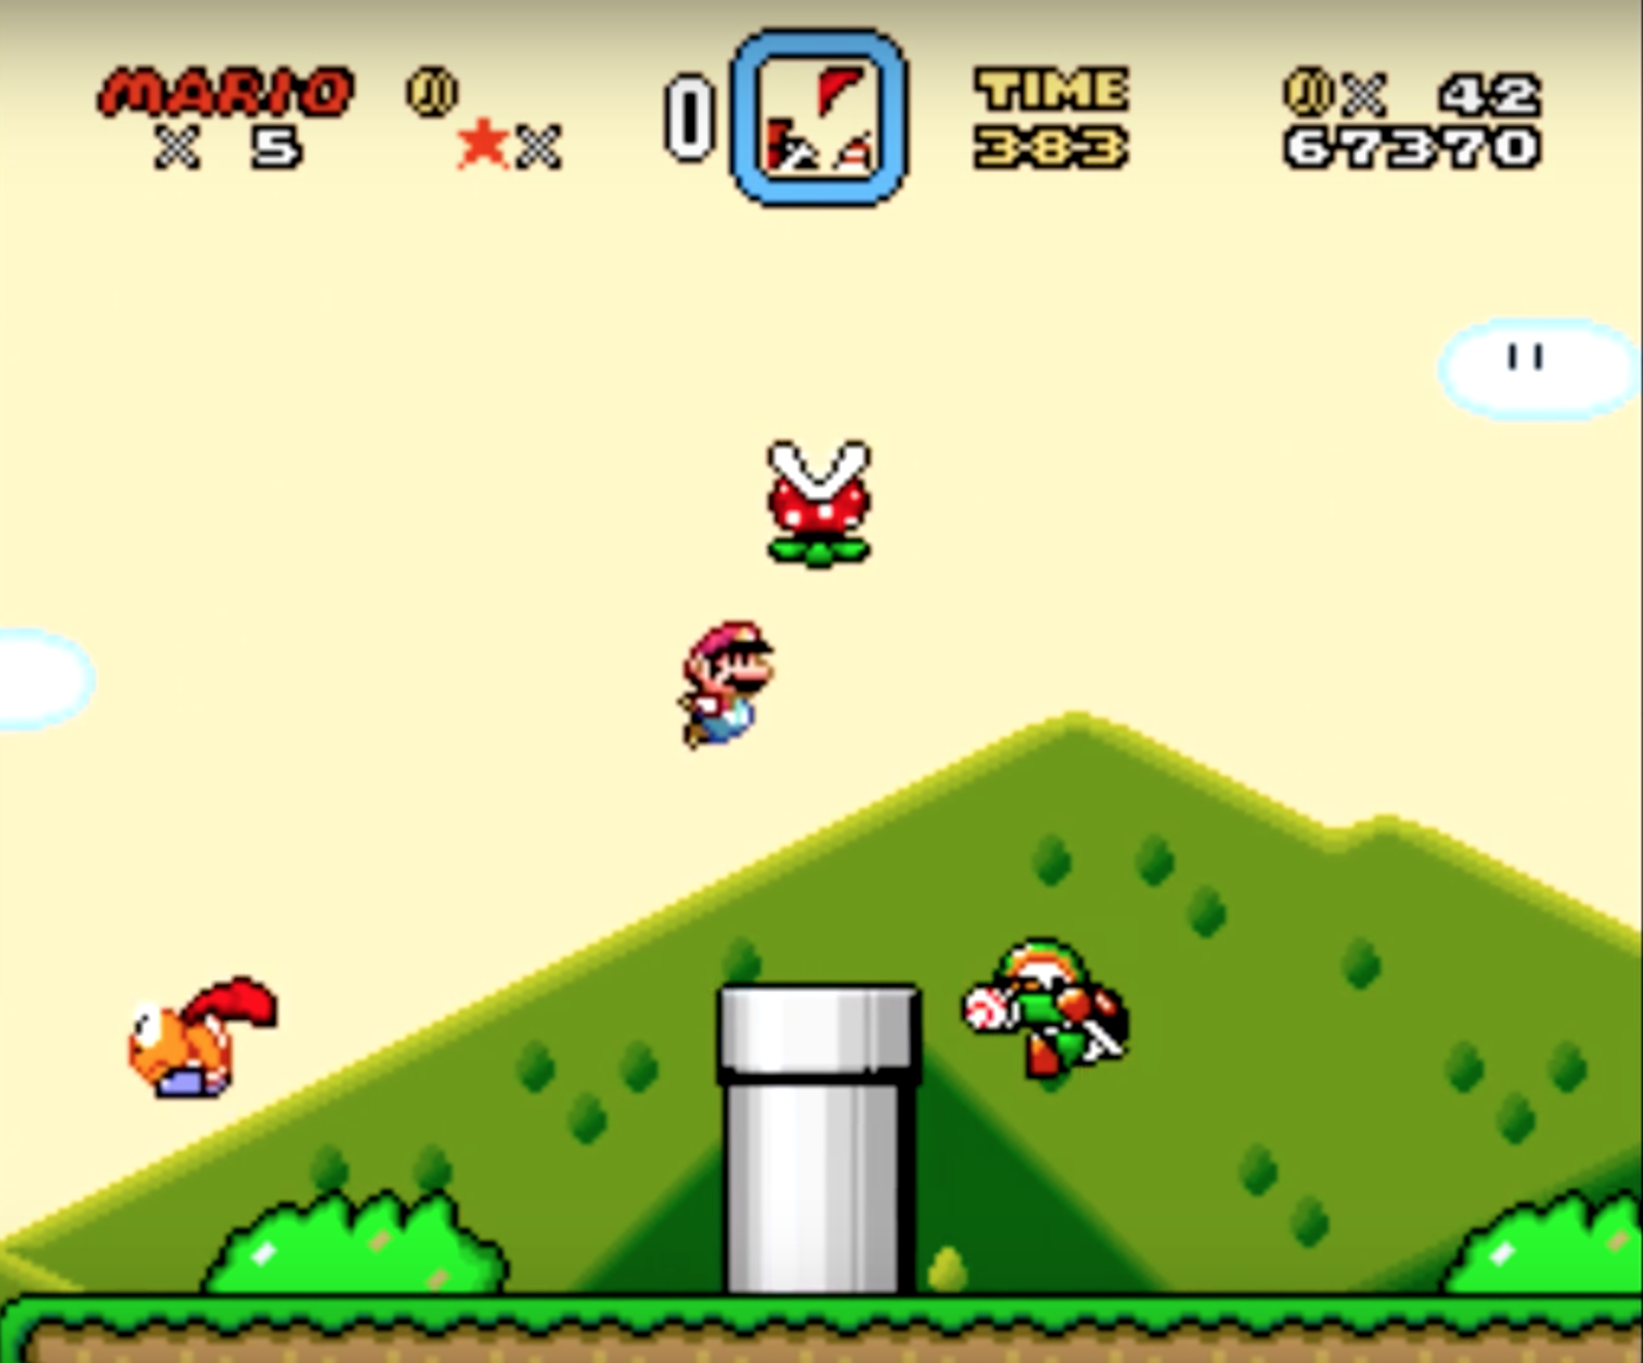
\includegraphics[width = \textwidth]{MarIO.png}
	\caption{MarI/O}
	\citep{MarIO} 
\end{figure}
%Probably need to ask for permission to use that 
%Sent a message on facebook to request permission

Despite that description, the intelligence of MarI/O is questionable. Although it has mastered the art of manoeuvring its way across the level in question, that is all it has done. In other words, if we were to take the same agent and run it on another Super Mario level, it would not do so well. It has figured out how to pass through the level by continually moving right, and jumping at optimal times to avoid enemies and gaps in the map. Albeit successful, this is not a strategy that could be deemed as \textit{intelligent}.

For Alan Turing to consider a machine intelligent, it must be able to act in a way that would be indistinguishable from the way a human would act. The Turing Test, created by Turing himself in 1950, was an imitation game whereby a human would hold textual conversations with another human, and with a computer. If the testing human is unable to successfully differentiate between the two based on interrogation within those conversations, then Turing would deem it unreasonable not to call the computer intelligent\citep{TuringTest}.

Although dealing in a different realm altogether, applying the same principle to MarI/O and questioning if the strategy it presents could pass a similar test of human judgement to decide whether or not it is a strategy that is likely to have been played by a human, then we cannot possibly declare MarI/O's technique as an intelligent solution.

Related videos include a Unity3D project that uses NeuroEvolution of Augmenting Technologies (NEAT) to teach a car model how to drive around a purpose-build track\citep{26}, and another neural network that plays Mario Kart 64\citep{27}. Furthermore, there is an interesting tutorial series entitled, \enquote{Python Plays: Grand Theft Auto V}\citep{28}, which makes use of TensorFlow\citep{17}.

%Particularly card games
\subsection{Why Neural Networks?}
This project has dealt a hand presenting a problem in which a decision making process will have to make use of imperfect information. Not only can neural networks cope with this, in fact, they excel in situations of imperfect information.

Without a neural network, any given scenario within a problem would need to have some kind of hard-coded solution that is step-by-step in nature. Through a learning process, a neural network can find solutions to these scenarios on its own, via exploration of the possibilities thrown up by its decision making process over several generations. 

Imagine having to write the code for a solution to every single possible game state in Chess. For every move, you would have to write a solution for it as many times as there are possible opportunities for that particular move, i.e, every possible board configuration in which that single move is legal. This would take an unthinkable amount of time, and in reality is probably not even possible. Providing a coded solution for every possible board configuration would require a huge amount of code segments declaring that if some state condition is true, then do move this piece to this location. In doing so, we would find ourselves with an enormous file size, requiring unrealistic amounts of memory to run the code. 

On top of that, it could take the machine a long time to search through all of the conditions to find the one that applies to the situation at hand. 

In Chess, there are 400 configurations possible after each player has made a single move each, and over 72,000 after two each\citep{20}. This continues to grow at an exponential rate, making it easy to see why implementing a fully coded strategy is unrealistic. Additionally, this renders using a search tree for exploration of the full search space infeasible\citep{29}. Using a neural network and allowing it to analyse every situation it encounters on its own, deciding what moves to make and learning from the results is a far better idea. 

Additionally, hard-coding solutions to given situations would make the game predictable, and could also lead to making moves that are not actually the best for that current game state. The flexible nature of a neural network provides the potential to reach better solutions that hard-coding might miss out on. 

In our Switch card game for example, there is a rule that states if the previous player played a 2, you must pick up two cards unless you have another 2. Knowing this, and wanting to force our opponent to inherit more cards, we might hard-code a strategy that says, \enquote{if you have a 2 and it is available to be played, play it.} This could cost an opportunity to win the game though. 

If we only had two cards left, both of the same suit and matching the suit of the most recently played card, one being a 2 and the other being a 7, we could play the 7 first, and that would allow us to play a run of that suit. This would allow us to play both cards and win the game. A neural network might learn that playing a 7 is better than deploying a 2, but our hard-coded strategy may not.

%*****what have people used neural networks for with control problems and how is it related to my problem******\\

Alter\citep{21} is another example implementation of artificial neural networks. Replicating the upper-body of a human, Alter is a robot that can almost be described as being \textit{alive}. 

Technologically, it consists of 42 pneumatic actuators and a \enquote{central pattern generator} with a neural network used to let the robot develop movement patterns\citep{21}. The network receives input in the form of sensory data relating to temperature and humidity as well as proximity and noise\citep{22}. 

Although it does not behave in a human-esque manner, Alter is continually perceiving the nearby environment, and reacting to it in such a way that is completely uncontrolled by a human, and not pre-programmed. This is how it somewhat provides the illusion of life. 

RoboCup\citep{23} is a robotics competition whereby robots compete in a game of football (soccer). The competition was launched by Japanese researchers in 1993, who soon after found themselves inundated with requests from other nations to make the project an international joint effort\citep{23}. 

RoboCup Soccer is an annual competition, and the performance of contestants is seen to increase across the various leagues yearly\citep{30}. Each league has a different type of robot, and so certain league alternate artificial intelligence problems with respect to the way in which they interpret and play the game. For example, not all of the leagues have robots with human-style bodies, and instead have wheels and 360$\degree$ vision. These variations allow for the RoboCup competition to encourage and facilitate research into an array of varying aspects within the artificial intelligence field. 

As the robots that participate in these competitions vary in size and shape, detecting fellow robots visually is not a simple task. It is however a job for a neural network of multi-layer perceptrons\citep{24}. Robots should also be able to recognise team-mates and tell them apart from opposing players. 

In terms of playing the game, it is infeasible due to the dynamic nature of the game to consider all situations ahead of time when programming the robot\citep{25}. Machine learning is therefore a necessity for RoboCup participation.

To demonstrate the significance of neural networks in the real world, here is a look at an open source software library that is used worldwide. 

Google initially developed TensorFlow, the successor to the DistBelief system they used from 2011\citep{19}, for research in neural networks and machine learning\citep{17}, but has since grown into a much wider-serving interface. It has found itself deployed in complex computational areas such as speech recognition and natural language processing, as well as image recognition\citep{18}. 

Google themselves use TensorFlow for a variety of different projects;  Massively Multitask Networks for Drug Discovery and RankBrain are examples of large-scale deep neural network projects owned by Google, used for drug discovery and information retrieval respectively\citep{17}. 

Other companies which benefit from the use of TensorFlow include Nvidia, Snapchat, Intel, Twitter, Dropbox, Ebay and Uber to name a few. \\

%RELATE IT TO A (CARD) GAME 

\subsection{Why Evolve Neural Networks?}
Artificial neural network evolution has demonstrated positive results with tasks involving reinforcement learning, and has performed especially well with those that include hidden state information\citep{EfficientEvolutionOfNeuralNetworkTopologies}. This appeals to the needs of this project as it deals with unknown game aspects, such as the cards in other people's hands. 

The evolution of neural networks has demonstrated a large degree of potential when coupled with tasks solvable by reinforcement learning techniques\citep{EfficientEvolutionOfNeuralNetworkTopologies}. It outperforms the basic methods of reinforcement learning against tasks that are considered benchmarks, and is therefore a justifiably sought after means of decision making.

Another arcade-style game that has been used in the research of neural networks is PAC-MAN. In a particular paper introducing the concept of trying to evolve a player for the retro classic, a simple ghost avoidance strategy was given a hard-coded implementation for comparison purposes. Perhaps expectedly, the results were underwhelming - in particular when compared to other implementations in the same project. The aim was to demonstrate that the neural networks were learning something more sophisticated than such a simple strategy\citep{MSPacMan}. Evolving neural networks and allowing the controller to develop its own strategies, as opposed to hard-coding them, produced universally superior results.

Evolved neural networks are not without disadvantages. Their black-box nature means that we do not get an understanding of why it makes certain decisions or takes particular actions, and it can be difficult to modify behaviours. Furthermore, there is the problem of potential overfitting, as previously described with the MarI/O\citep{MarIO} example where the agent has perfected that particular Mario map, but if it were to be placed in a new environment, the same strategy would not suffice. It would be the same as introducing a robot of never before seen size or shape in our RoboCup\citep{24} example, without allowing retraining with images of the new robot machine.\\

\subsection{Why Co-Evolve Topologies and Weights?}
Much like when we compare evolving neural networks to standard reinforcement learning techniques, evolving network topologies often performs in a significantly superior manner to the alternative - in this case fixed topology neural network evolution\citep{EfficientEvolutionOfNeuralNetworkTopologies}. 

There is always a chance with evolving topologies of making the search overly complex, but in contrast to that possibility there is also the potential to find the optimal amount of hidden nodes for any given problem by itself, which would save some time\citep{EfficientEvolutionOfNeuralNetworkTopologies}. It is also possible for NEAT to reduce the complexity of a network's structure when evolving the topology. 

Rather than searching through topology space using a brute force approach, NEAT begins with small, simple networks before expanding the search space only when necessary\citep{EvolvingARovingEyeForGo}. This strategy attempts to counter the problem of overfitting, and the flexibility is what allows it to find far more complex controllers than evolution networks with a non-negotiable topology.\\

%RELATE IT TO A (CARD) GAME \\

\subsection{Summary}
%Given previous work it suggests that NEAT will be an appropriate algorithm for solving this problem
%The unanswered questions (that we will go on to answer):
%-How intelligent is the solution
%-How many generations did it take
%-How computationally complex is it regarding hidden layers and topology. 
Evolving artificial neural networks, including structural network evolution, allows us to create solutions that perhaps would not be feasible to build with step-by-step hard-coding approaches. For a project such as this where we cannot write a fool-proof strategy to deal with any given situation within the game, it is ideal to have tools such as NEAT. 

Despite the disadvantages and complexities of evolved neural networks, the negatives are outweighed by positives. They are able to achieve things that developers alone cannot, and so it would be difficult and perhaps unwise to overlook them for some projects, particularly those with huge search spaces like Chess and Go.  

As Switch is largely down to luck like most (if not all) card games, there is never going to be a perfect solution. That said, the aim of this project is to see whether evolved neural networks are more capable of finding a consistently positive solution than a programmer implementing a strategy in advance could be. 

\newpage
\section{Rules of Switch}
Before proceeding to discuss the inner workings of the digital version, it may help to explain how the game works physically.

The objective of Switch is to be the first player to successfully empty their hand of cards, although the game can - and in this case does - continue until all players - except last place - has done so. Players are equally dealt a number of cards, before the card on top of the stack is turned over to reveal its type and suit. 

The player left (or right if the upturned card was a Jack) of the dealer must then play a card which matches in either type or suit. An inability to do so results in the current player adding a new card from the top of the pack into their hand. The next player on the left must then do the same, and play continues in this vein.

Of course, there is more to it than that. Certain cards have rules attached to them. Not all of the rules played in real life are (fully) implemented into this project. To avoid confusion, only the rules associated with the project will be explained here; A more inclusive explanation can be seen on my website (Appendix E).\\

The special cards are as follows:
\begin{itemize}
	\item Black Queen
	\item Two
	\item Eight
	\item Jack
\end{itemize}

A Queen of either Clubs or Spades will result in the next player having to pick up five cards, and any Two forces an addition of two cards. Playing an Eight means your next opposing player skips a turn, and a Jack will switch the direction of play. 


\newpage
\section{Methodology}
%The entire project source code can be found on \href{http://www.github.com/x4iiiis/honoursproject}{my github account.}


\subsection{Language and Libraries}
The software development language used to build this project is C++. It is used in collaboration with the NeuroEvolution of Augmenting Topologies (NEAT) library. In order to run the application, compatibility with C++11 is necessary of the user's chosen compiler, due to the use of shared pointers - a relatively modern development concept. 

When working with NEAT, documentation including a tutorial on how to write new experiments was observed(Appendix G). 

The graphical aspect of the game on show in Figure 10 was implemented using an import of the Simple and Fast Multimedia Library (SFML), with playing card textures courtesy of Kenney Vleugels (Appendix F).\\

\begin{figure}[h]
	\centering
	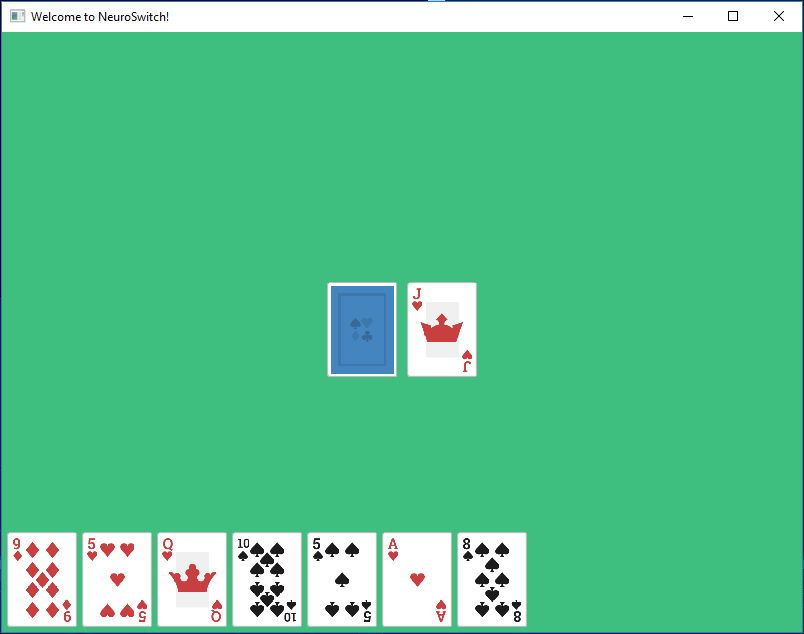
\includegraphics[scale = 0.6]{SFML.png}
	\caption{Game UI}
\end{figure}

\newpage
\subsection{Design}
%Design patterns / class diagrams and such for my code
%An object oriented approach to the programming of this game made sense as the intention was to replicate a game that was physically played in the real world. Thinking of the digital version in the same way as the real world game 

\begin{figure}[h!]
	\centering
	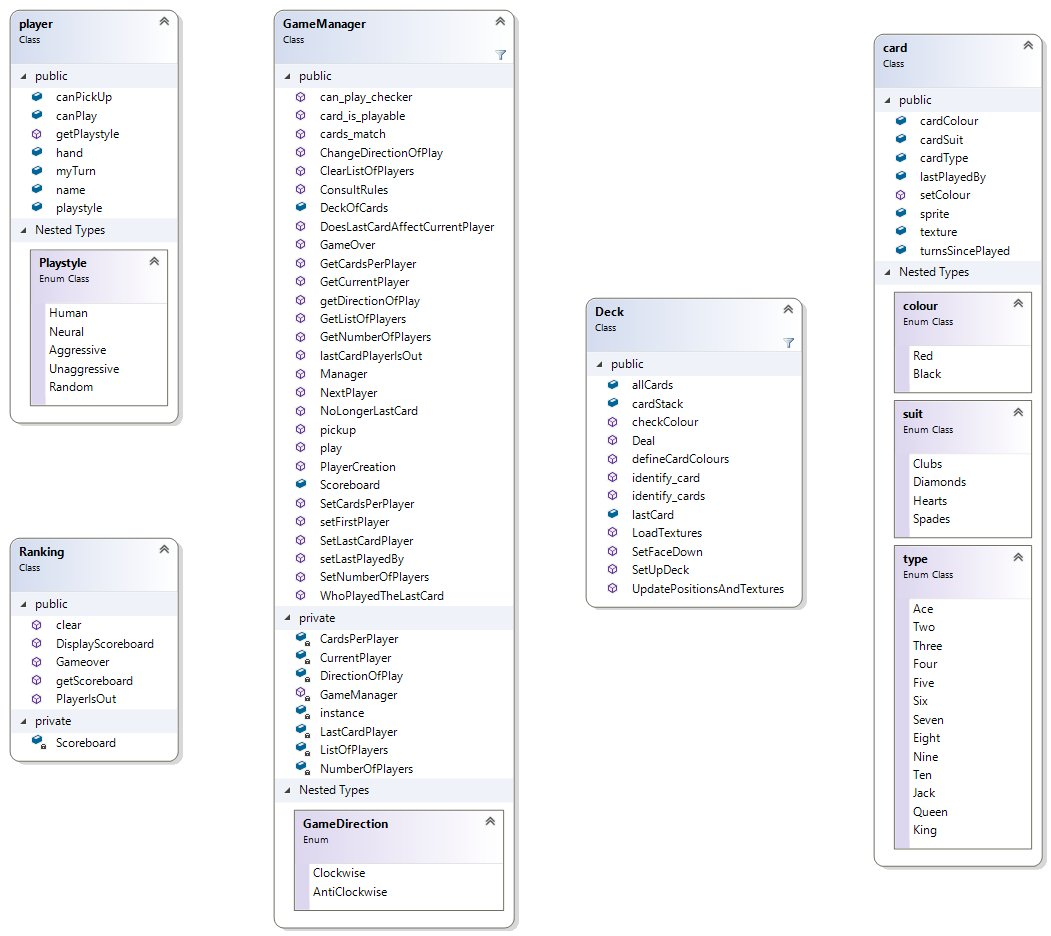
\includegraphics[width = \textwidth, height = 400pt]{ClassDiagram.jpg}
	\caption{Game Class Diagram}
\end{figure}

Figure 11 helps to visualise the code structure behind the game, showing the five classes and their member functions. 

The Game Manager class is central, with its deck of cards object class on the right. For the sake space and readability, 105 card and texture objects have been omitted from the image. The specifics of what a card object is made up of can be seen on the far right. Also pictured, we see the ranking system and a look at the components of a player object.

As seen in the diagram, the game management class is the hub that interacts with everything throughout each match. It is an integral part of the game operation, and needed to be reliable. For example, if a bug was existed where a second game manager was created with some functions referencing the first instance, and other methods using the second, then the game would jump around as the states of the two decks would be different. While this would most likely cause the program to crash anyway, it was good to know it was not going to happen when the class was converted to a singleton.

A singleton is a software engineering design pattern used to eliminate the risk of accidentally duplicating the existence of an object that is only meant to be instantiated once in an application\citep{31}. To achieve this, the function call whereby an object of this type would be created first checks to see if an instance already exists. If it does, then the function returns access to the existing version of the object. If the object instance is set to null, then it is yet to be created, and the creation process can then go ahead.

The singleton pattern was at one stage thought to be essential to the development of this project, but was later realised as slightly unnecessary. However, there is no harm in keeping it.

Player and card objects are used across multiple classes in the game code via the use of shared pointers. \enquote{The shared\_ptr type is a smart pointer in the C++ standard library that is designed for scenarios in which more than one owner might have to manage the lifetime of the object in memory\citep{sharedptr}.} Introduced in C++11, shared pointers are a relatively new concept, and so a modern compiler is required to execute the game. This created a few issues when interfacing with the NEAT library, whose code was written over fifteen years ago. \\

\subsection{Game}
The game manager class creates a ranking system, and a deck of cards. The ranking class is very simple. It is merely an external object to keep track of the scoreboard, by storing the players that have successfully got out of the game. It is also used to check if the game is over. The class method is passed a value describing the amount of players that started the game, which it then compares to the count of players currently in its scoreboard. If the difference between the two values leaves a single player alone in the game, then the game is over, and that player is also added to the scoreboard in last place. This scoreboard is then displayed on screen in the console, and printed to file.

The deck creates and stores all of the card objects, and is responsible for their textures and positions on screen, and is also the class responsible for keeping track of the stack and last played card. The game manager carries out some tasks via the deck object too. These methods did not necessarily need to be in the deck object; Having them there just made it simpler to keep card and deck related methods together when developing the system. The most important example of this is the deal method, used for distributing the cards to the players at the beginning of a game.

Game.h, the main file used to run games, is where the game manager is created. Once it has been instantiated, the game class then gets the game manager to create the players and set their names and play-styles, before then dealing the cards. Once the cards have been dished out and the first card to be played on is known, the program enters the game loop. Once in this phase of the application, the same segment of code is repeatedly executed until the game-over criteria of the ranking system has been reached. 

The loop contains conditional statements used to determine which type (play-style) of player the current turn belongs to. Then the system will check whether or not the current player can legally play a card. If not, the player will have to pick up, and non-human players will automatically do so. Otherwise, play-style specific mechanics are in place for moves to be made. Each time a move is made or a card is picked up, the game manager ends the turn of that player and moves on to the next, making a quick call to the scoreboard to ensure that the game is not yet complete, before the game class returns to the beginning of the loop. When that game-over check returns a positive result, the loop is broken and the game is terminated; returning the fitness of any existing neural players to the NEAT code.

An issue that arose when the game was hooked up to the NEAT library was that the random function used to shuffle the cards before dealing is not does not produce authentic random results. The generator is seeded by the current time at which it is called, down to the present second. When the graphical aspect of the game was removed, the need for a pause between each play to allow the user to see what happened went with it, and what remained was a very fast, console-based application. So fast, in fact, several tens of games can be completed in a single second. This presents a problem as the pseudo-random dealing of cards is seeded to a single second. Thus, any games sharing a second of time when cards are dealt consequentially result in the players receiving exactly the same first hand, and the same first card to play on top of. It is highly probable that these games should result in the same outcome. 

This can easily be overcome by allowing the process to pause for a second after each game, but this drastically increases the time taken to obtain results from larger populations and multiple generations. Instead, a decision to pause after each generation was taken. This means that several - and potentially all - members of the population are playing games with the same initial game states. This invariably results in some games playing out in exactly the same way, but as the population evolves, organisms will make differing decisions in scenarios where more than one potential move is available to them. Of course, even one variation in card choice alters the entire game trajectory from that point onwards, and so as long as a situation arises where a choice can occur, the \textit{exact} same game is less probable. 

In a way, this makes judgement of generational results slightly less harsh, as similar games were played and the actions resulted differently.\\


\subsection{Neural Network}
Whilst a possibility, building a neural network from scratch was an option that was given little consideration due to the lack of knowledge in the field already evident at the beginning of the project. Using pre-built and thoroughly documented software allowed for more time to be allocated to the development of the game structure, and experimenting with neuro-evolution techniques more freely. The project was intended to be primarily about developing the game and analysing results obtained by evolving a neural network over a significant number of games. 

In early stages of development, it was thought that there would be a long period where the network would have to learn how to play the game. With this, it was suspected that a means to recognise and punish illegal move attempts. However, an alternative was implemented. Each time the game loops back around to the Neural player's turn, the entire first layer of input nodes is reset to -10, before then stepping through their hand one card at a time, calling a method in the game manager class to determine whether or not the current card is playable against the most recently played card. Assigning a value of 1 to the corresponding node for cards that receive a positive response from the legality-checking function in this manner then allows the network to choose from the set of cards it is allowed to play.

The network then runs through all of the output nodes, seeking the node with the greatest activation. Once this node has been discovered, a large switch case function is in place to actually make the move for the network, using the card that relates to the most activated output node. 

If unable to play due to having no playable cards available, the Neural player will automatically pick up a card without bothering the network.

Creating the network for this project was a straightforward procedure of setting 52 input nodes, and 52 output nodes. Each card in the deck corresponds to one of each node type. Node 1 relates to the Ace of Clubs, and so does node 53 (the first output node). 

\newpage
\subsection{Evolutionary Algorithm}
\begin{figure}[h!] 
	\centering
	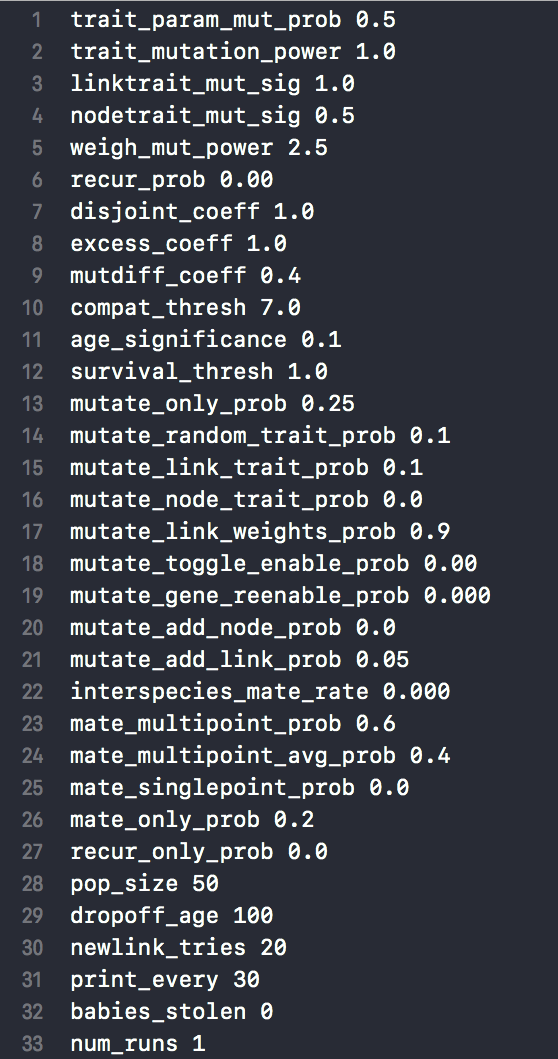
\includegraphics[width = \textwidth/2]{neFile.png}
	\caption{NeuroSwitch.ne}
\end{figure}

Figure 12 contains the variables available to be tampered with when using NEAT. The library reads this file in, and uses it to evolve the neural network as experiments are executed. 

As NEAT takes care of the reproduction work, this input file is as close as the project got to that level. The \enquote{survival\_thresh} variable relates to the fitness function in the upcoming subsection, and \enquote{pop\_size} is how many members are in the population. Setting \enquote{mutate\_add\_node\_prob} to 0 ensured that the network structure remained the same, as having more input or output nodes than cards would have the potential to break the game. 

Most of the other variables can be used to experiment with the evolution of the population. 


\newpage
\subsection{Fitness Evaluation}
A fitness function was always going to be a challenge with this project. The stochastic nature of the game makes evaluating performance extremely difficult. One idea was to reward the neural player for playing cards that would negatively influence the opposition. This was promptly counter-thought as that would promote playing aggressively. Whilst this may not be a bad thing, it would almost create an elaborate replicate of the hard-coded aggressive player. 

Another thought was to negatively affect the fitness every time the player's hand increased in size. However, the unpredictability of would often lead to negative fitness values - even if the player won the game. There was briefly an attempt to counteract this with large increases or decreases when the game ends - depending on whether or not the neural player won or lost. This was insufficient as the length of games varies every time, so the effect of the counterweight fluctuated.

In the end, fitness was simply evaluated in a binary fashion; Win or loss. The survival threshold for organisms in the population of a generation was later set so that only winning members survived. This seems harsh as the player could theoretically perform exceptionally well in one game, only to be dealt a poor hand in its next match and be terminated as a result. However, an alternative was difficult to come by.



\newpage
\section{Results}
%Hardcoded stuff\\\\
When the underlying game foundation had been built, it only allowed for human vs human interaction. This meant testing was not only very click-intensive, but also extremely time consuming. As a result, some automatic playability was implemented to allow for speedy, hands-free testing. The automatic players were given hard-coded strategies for playing the game, aptly named, `Aggressive,' `Unaggressive,' and `Random.' 

The aggressive player will check their hand for cards that will inflict the most damage to their opponents, before just selecting the first legal card in the hand if none are available. Unaggressive does the opposite. It actively avoids playing twos, eights and black queens unless no other playable cards are contained in their hand. Random players will just shuffle their hand before choosing a playable card.

Once the game had been thoroughly tested and all bugs eradicated, work on the final player type was to ready to be begin. Of course, the `Neural' player was going to be playing against the hard-coded play-styles, as well as potentially facing humans in future. For this reason, a baseline of hard-coded performances was measured. The strategies were tested against one another in a one on one format, before a free for all between the three.\\

Below are a series of tables depicting the results of this testing.\\

\begin{table}[h!]
	\begin{tabu} to \textwidth { | X[c] | X[c] | X[c] | }
		\hline
		Games Played & Aggressive Wins & Unaggressive Wins \\
		\hline
		1000  & 552	& 448 \\
		\hline
	\end{tabu}
\caption{Hard-coded Results | Aggressive vs Unaggressive}
\label{table:1}
\end{table}

\begin{table}[h!]
	\begin{tabu} to \textwidth { | X[c] | X[c] | X[c] | }
		\hline
		Games Played & Aggressive Wins & Random Wins \\
		\hline
		1000  & 501 & 499 \\
		\hline
	\end{tabu}
\caption{Hard-coded Results | Aggressive vs Random}
\label{table:2}
\end{table}

\begin{table}[h!]
	\begin{tabu} to \textwidth { | X[c] | X[c] | X[c] | }
		\hline
		Games Played & Random Wins & Unaggressive Wins \\
		\hline
		1000  & 539 & 461 \\
		\hline
	\end{tabu}
\caption{Hard-coded Results | Random vs Unaggressive}
\label{table:3}
\end{table}

As expected, the more attacking player had the most success. However, I was taken aback to discover it only won 55.2\% of 1000 games against the unaggressive player affectionately known as `Passive Pete.' This was less surprising than the difference between 	`Angry Adalia' and `Random Rachel' however. I had predicted a landslide victory for aggressive, but had the random strategy won just a single game more, it would have been a tie over 1000 iterations. I think these results in particular are testament to the unpredictability of Switch. 

The remaining battle was between Random Rachel and Passive Pete. There is not a lot to be said about this. An unaggressive approach to the game is effectively allowing the opposition to play without being severely punished, and deserves to yield poor results. Similarly, the random approach is totally unpredictable, and so this contest could probably go either way if repeatedly tested.\\

Finally, the ultimate showdown; Aggressive vs Unaggressive vs Random. 

\begin{table}[h!]
	\begin{tabu} to \textwidth { | X[c] | X[c] | X[c] | X[c] |}
		\hline
		Games Played & Aggressive Wins & Unaggressive Wins & Random Wins\\
		\hline
		1000  & 346	& 314 & 340 \\
		\hline
	\end{tabu}
	\caption{Hardcoded Results | Aggressive vs Unaggressive vs Random}
	\label{table:4}
\end{table}

As the results show, the aggressive play-style is the most successful. However, the margin of victory was somewhat surprising.\\

\subsection{Network vs Hard-coded Strategy}
The following tables show the average results of each generation performing against the stated hard-coded play-style. Each generation consists of the following:

\begin{itemize}
	\item Population of 20 (pre-dropoff)
	\item Dropoff age of 100
	\item 1 run per member of population
\end{itemize}

Averages are calculated from 10 replicates of the same tests. \\\\

\begin{small}
	\textit{Tables show only the averages of every 5th generation to ensure only a single page of space is required. The full dataset is available on my website(Appendix E).}
\end{small}

\newpage
\subsubsection{Neural vs Unaggressive}

\begin{table}[h!]
	\begin{tabu} to \textwidth { | X[c] | X[c] | X[c] |}
		\hline
		Generation & Population Size & Average Wins \\
		\hline
		1  & 20  &  11.9\\
		\hline
		5  & 20 & 11.8\\
		\hline
		10 & 20 &  9.6\\
		\hline
		15 & 20 & 10.9\\
		\hline
		20  & 20 & 8.7\\
		\hline
		25  & 20 & 11.1\\
		\hline
		30  & 20 & 13\\
		\hline
		35  & 20 & 11.4\\
		\hline
		40  & 20 & 10\\
		\hline
		45  & 20 & 11.2\\
		\hline
		50  & 20 & 12.1\\
		\hline
		55  & 20 & 11.4\\
		\hline
		60  & 20 & 11.5\\
		\hline
		65  & 20 & 11.2\\
		\hline
		70  & 20 & 11\\
		\hline
		75  & 20 & 9.4\\
		\hline
		80  & 20 & 13.1\\
		\hline
		85  & 20 & 8.9\\
		\hline
		90  & 20 & 5.3\\
		\hline
		95  & 20 & 5\\
		\hline
		100  & 20 & 6.2\\
		\hline
		105  & 20 & 5.5\\
		\hline
		110  & 10 & 5\\
		\hline
		115  & 10 & 6.2\\
		\hline
		120  & 10 & 5.5\\
		\hline
		125  & 10 & 5\\
		\hline
		130  & 10 & 5\\
		\hline
		135  & 10 & 6.9\\
		\hline
		140  & 10 & 5.1\\
		\hline
		145  & 10 & 5.2\\
		\hline
		150  & 10 & 6\\
		\hline
	\end{tabu}
	\caption{Average Results | Neural vs Unaggressive}
	\label{table:5}
\end{table}

\begin{figure}[h]
	\centering
	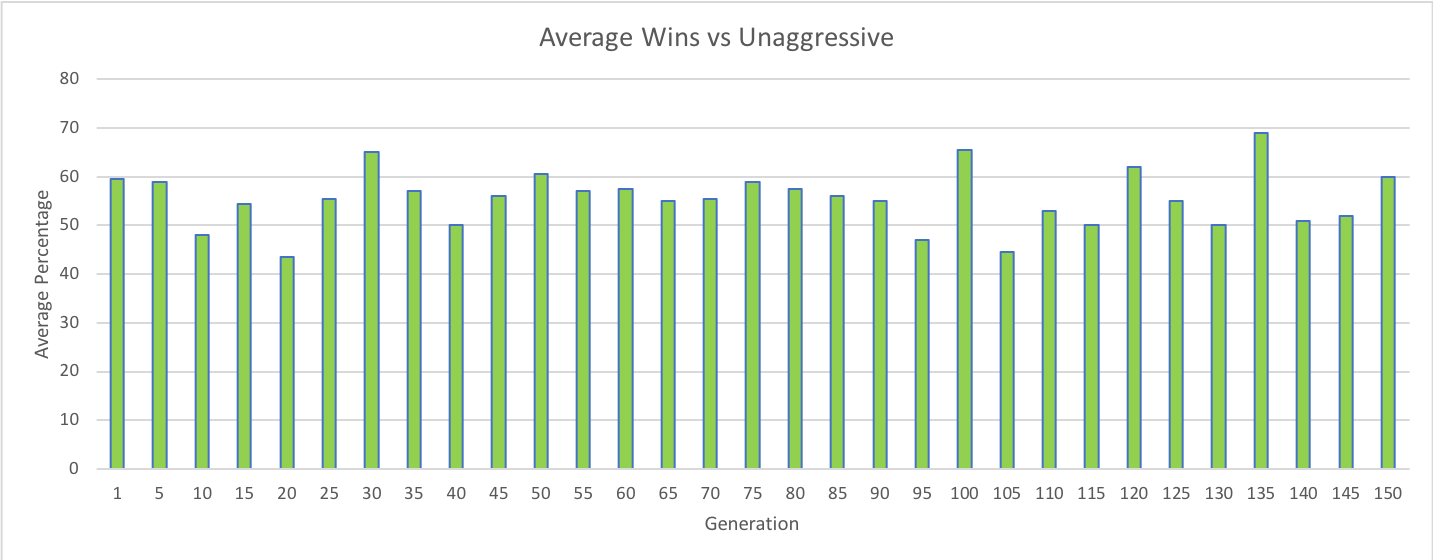
\includegraphics[width = \textwidth]{Una1.png}
	\caption{Average Results vs Unaggressive}
\end{figure}

\newpage
These average results affirm scepticism about the likelihood of any consistency in terms of machine learning and progressive improvement in performance. However, these results show that the neural players were winning the majority of their generation's games, with the exception of a handful. It is important to remember that the unaggressive player is less likely to play cards that significantly hinder the chances of neural success, though.

\subsubsection{Neural vs Random}
When the network took on the random strategy, it appears to have played worse on average than it did in the previous results. With the exception of a single sub-30\% generation, the average does not stray far below the 50\% win rate. Again, there are no exceptionally successful generations. However, the unpredictability may present a mildly more authentic opponent.

\begin{figure}[h]
	\centering
	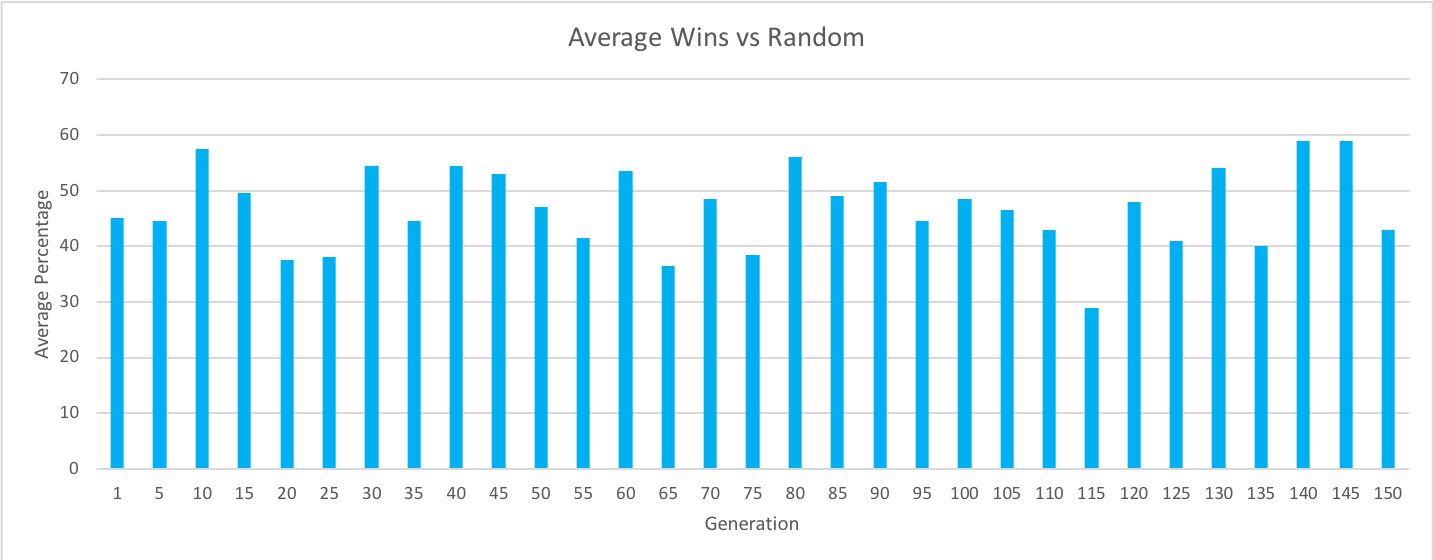
\includegraphics[width = \textwidth]{Rand1.png}
	\caption{Average Results vs Random}
\end{figure}

\newpage
\begin{table}[h!]
	\begin{tabu} to \textwidth { | X[c] | X[c] | X[c] |}
		\hline
		Generation & Population Size & Average Wins \\
		\hline
		1  & 20  & 9 \\
		\hline
		5  & 20 & 8.9\\
		\hline
		10 & 20 & 11.5\\
		\hline
		15 & 20 & 9.9\\
		\hline
		20  & 20 &7.5\\
		\hline
		25  & 20 &7.6 \\
		\hline
		30  & 20 & 10.9\\
		\hline
		35  & 20 & 8.9\\
		\hline
		40  & 20 &  10.9\\
		\hline
		45  & 20 & 10.6\\
		\hline
		50  & 20 &9.4 \\
		\hline
		55  & 20 &8.3 \\
		\hline
		60  & 20 &10.7\\
		\hline
		65  & 20 &7.3\\
		\hline
		70  & 20 &9.7 \\
		\hline
		75  & 20 &7.7 \\
		\hline
		80  & 20 & 11.2\\
		\hline
		85  & 20 & 9.8 \\
		\hline
		90  & 20 & 10.3\\
		\hline
		95  & 20 &8.9 \\
		\hline
		100  & 20 &9.7 \\
		\hline
		105  & 20 &9.3 \\
		\hline
		110  & 10 & 4.3\\
		\hline
		115  & 10 &2.9 \\
		\hline
		120  & 10 &4.8 \\
		\hline
		125  & 10 & 4.1\\
		\hline
		130  & 10 & 5.4\\
		\hline
		135  & 10 & 4\\
		\hline
		140  & 10 &5.9 \\
		\hline
		145  & 10 & 5.9 \\
		\hline
		150  & 10 & 4.3\\
		\hline
	\end{tabu}
	\caption{Average Results | Neural vs Random}
	\label{table:6}
\end{table}


\newpage
\subsubsection{Neural vs Aggressive}
\begin{table}[h!]
	\begin{tabu} to \textwidth { | X[c] | X[c] | X[c] |}
		\hline
		Generation & Population Size & Average Wins \\
		\hline
		1  & 20  & 9.2 \\
		\hline
		5  & 20 & 10.1\\
		\hline
		10 & 20 &  10.1\\
		\hline
		15 & 20 & 8.7\\
		\hline
		20  & 20 & 10.2\\
		\hline
		25  & 20 & 9.4\\
		\hline
		30  & 20 & 9.3\\
		\hline
		35  & 20 & 7.7 \\
		\hline
		40  & 20 & 11.5\\
		\hline
		45  & 20 & 9.1 \\
		\hline
		50  & 20 & 6.8 \\
		\hline
		55  & 20 & 9.4\\
		\hline
		60  & 20 & 7.2\\
		\hline
		65  & 20 & 8.6\\
		\hline
		70  & 20 & 8.7\\
		\hline
		75  & 20 & 10.4\\
		\hline
		80  & 20 & 9.4\\
		\hline
		85  & 20 & 9.7\\
		\hline
		90  & 20 & 9.8\\
		\hline
		95  & 20 & 8.7\\
		\hline
		100  & 20 & 10\\
		\hline
		105  & 20 & 10\\
		\hline
		110  & 10 & 4\\
		\hline
		115  & 10 & 4.7\\
		\hline
		120  & 10 & 4.7 \\
		\hline
		125  & 10 & 4.4 \\
		\hline
		130  & 10 & 4.5 \\
		\hline
		135  & 10 & 3.4 \\
		\hline
		140  & 10 & 3.9 \\
		\hline
		145  & 10 & 6.6\\
		\hline
		150  & 10 & 4.2\\
		\hline
	\end{tabu}
	\caption{Average Results | Neural vs Aggressive}
	\label{table:7}
\end{table}

\newpage
The attacking nature of this opponent made it the most likely to hurt the network's success rate. The data concurs, as almost all of the generations won less than half of their games on average. Interestingly, one of the later generations broke the trend with some consistently high win rates, but the huge drop from that generation to five generations later suggests that this was coincidental good fortune.

\begin{figure}[h]
	\centering
	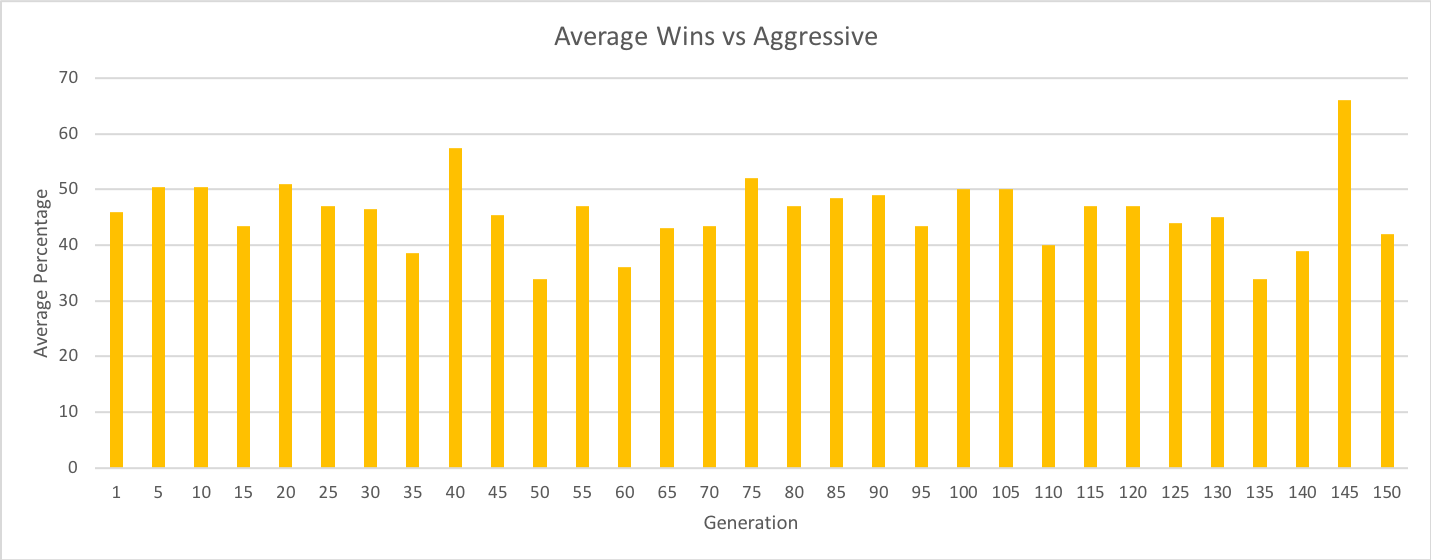
\includegraphics[width = \textwidth]{Agg1.png}
	\caption{Average Results vs Aggressive}
\end{figure}

%\newpage
%\subsubsection{Free For All }
%Every radge for eezsel

%Just do a pretty short, 1 replicate, fatal four way thing
%. . . . . . . 
\begin{small}
	\begin{center}
		\textit{All results can be downloaded from my website (Appendix E).}
	\end{center}
\end{small}

\subsection{Deeper Examination}
Graphing the average win rate merely shows that success fluctuates across the range, largely due to the stochastic nature of the card game at hand. 

\begin{figure}[h]
	\centering
	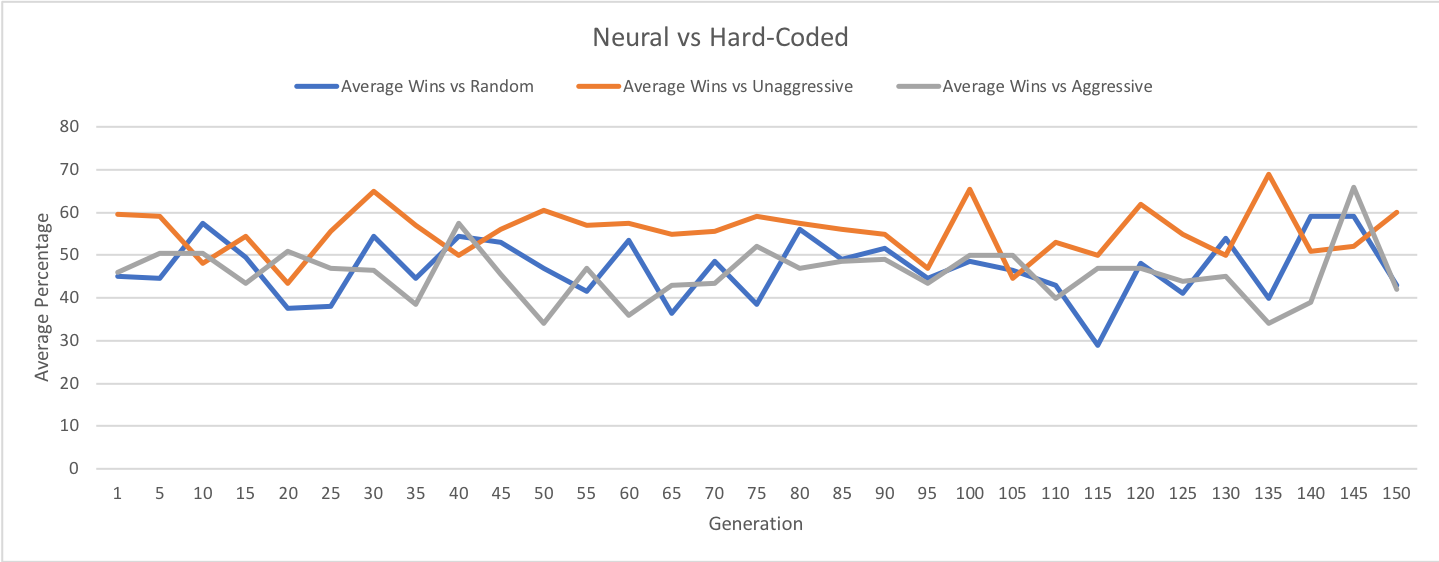
\includegraphics[width = \textwidth]{ComparisonLineGraph.png}
	\caption{Neural vs Hard-Coded Comparison}
\end{figure}

Using box charts to further investigate the results provides more interesting information about the games. However, while this new evaluative approach delves more into the success rate of generations, the set needed to be more sparse for the sake of graph readability. Thus, the generations are split quarterly to one hundred, including the first generation. 

The height of each box indicates the standard deviation of the corresponding generation. Simply put, standard deviation is a means of calculating the variance from the average across all of the values - in this case games won. The horizontal line across the boxes represent the (previously inspected) median, and the lines attached to the vertical line through the centre are error bars; Used to represent extremes and uncertainty of the dataset. The circles are the actual values.

\newpage
\begin{figure}[h]
	\centering
	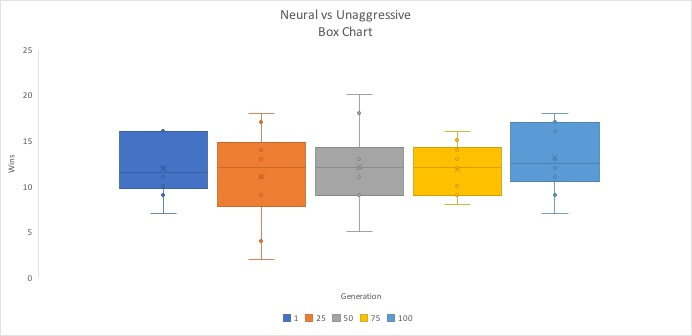
\includegraphics[width = \textwidth]{BoxUna.jpg}
	\caption{Box Chart | Neural vs Unaggressive}
\end{figure}

Despite the fact that there are 24 missing generations between each box, there appears to be a trend with the unaggressive opposition. It looks as if the generations became more consistent. Albeit in a less-successful manner, it appears that the variety across experiments was reduced over time. 

\begin{figure}[h]
	\centering
	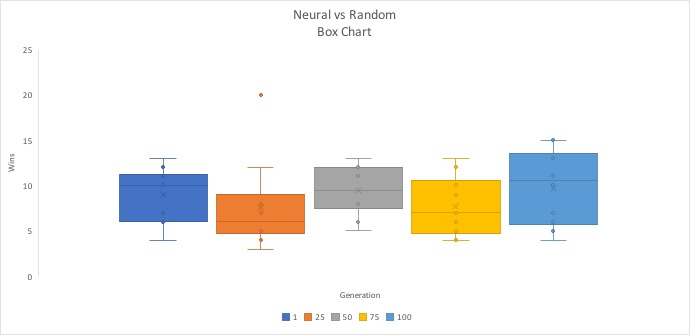
\includegraphics[width = \textwidth]{BoxRand.jpg}
	\caption{Box Chart | Neural vs Random}
\end{figure}

The random chart is interesting. Taking a look at generation 25, average performance was below 50\%. Despite this, one of the replicates of this experiment won all 20 games. This generation is the only one pictured with an outlier. Had there been a trend of highly successful outliers across the graph, perhaps there would be an argument that it is possible to perform strongly in a consistent manner, or that the network had maintained a plausible strategy. This is unfortunately not the case though, as the graph shows that even that collection of games dropped back down to a lower win rate and managed to blend in with the other results.

\begin{figure}[h]
	\centering
	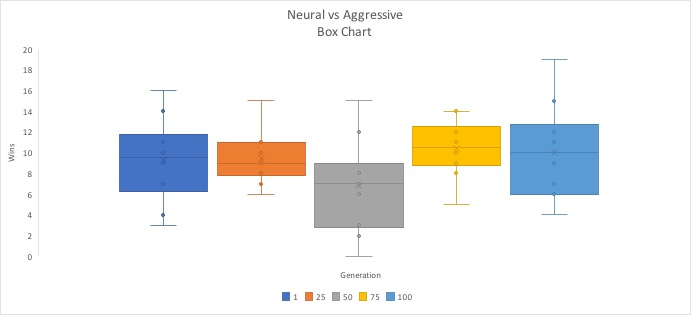
\includegraphics[width = \textwidth]{BoxAgg.jpg}
	\caption{Box Chart | Neural vs Aggressive}
\end{figure}

Eyes are immediately drawn to the 50th generation in the aggressive chart. Worse off than the 1st and 25th generation, our middle box shows a real dip in form for the neural player when taking on aggressive opposition. The extremes also show large fluctuation, including a generation that lost every game. 

Losing every game would result in a complete rebuild in the population, and so the next generations would be expected to perform poorly too.\\ 

Breaking down the gap in the graph, relative to the winless experiment:

\begin{table}[h!]
	\begin{tabu} to \textwidth { | X[c] | X[c] | X[c] |}
		\hline
		Generation & Population Size & Wins \\
		\hline
		55  & 20  & 14 \\
		\hline
		60 & 20 & 3\\
		\hline
		65 & 20 & 5\\
		\hline
		70 & 20 & 13\\
		\hline
	\end{tabu}
	\caption{Investigating Aggressive Extremes}
	\label{table:8}
\end{table}

Unsurprisingly, the stochastic nature of dealing cards in the beginning of games has thoroughly skewed the data.

\newpage
\subsection{Evolution | Mating vs Mutating}
As seen in Figure 12, the NeuroEvolution input file had a \enquote{mate only probability} value of 0.2, and a \enquote{mutate only probability} of 0.25. These variables were experimented with in this subsection. Creating a 75\% to 25\% split in produced the following charts.  
%\newpage
\subsubsection{Comparison | Unaggressive}

%Have these two figures next to each other
\begin{figure}[h]
	\centering
	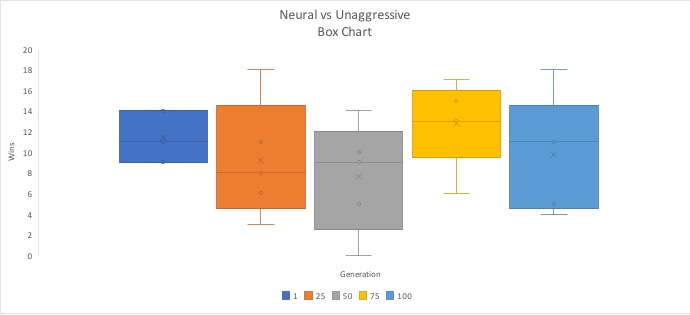
\includegraphics[width = \textwidth]{BoxUna2.jpg}
	\caption{Box Chart | Neural vs Unaggressive | Mating }
\end{figure}

\begin{figure}[h]
	\centering
	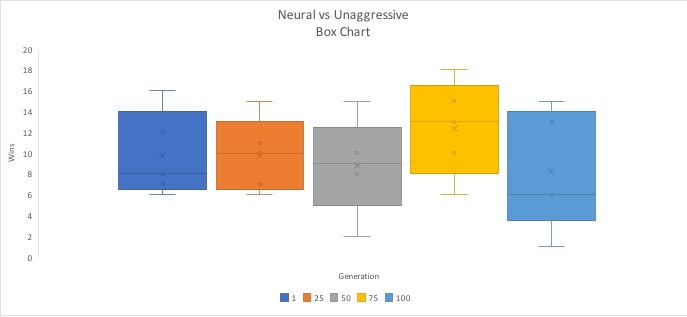
\includegraphics[width = \textwidth]{BoxUna3.jpg}
	\caption{Box Chart | Neural vs Unaggressive | Mutation}
\end{figure}

In terms of the diagram flow, the two are very similar. In the mutation tests, generation 25 did better than in the mating example, while the 100th generation did more poorly.

Although nothing to do with the evolution, the first generation gathered results in a more confined range in the first graph, but then created a diverse range by the 25th generation, whereas the mutation example maintained a similar standard deviation throughout, with the exception of the final box in the graph, which shows considerable expansion by contrast.  

%\newpage
\subsubsection{Comparison | Aggressive}

\begin{figure}[h]
	\centering
	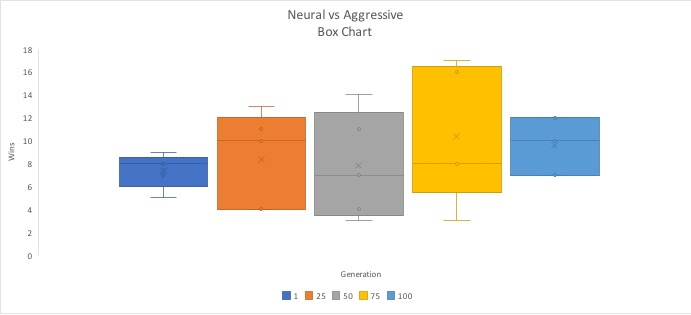
\includegraphics[width = \textwidth]{BoxAgg2.jpg}
	\caption{Box Chart | Neural vs Aggressive | Mating}
\end{figure}

\begin{figure}[h]
	\centering
	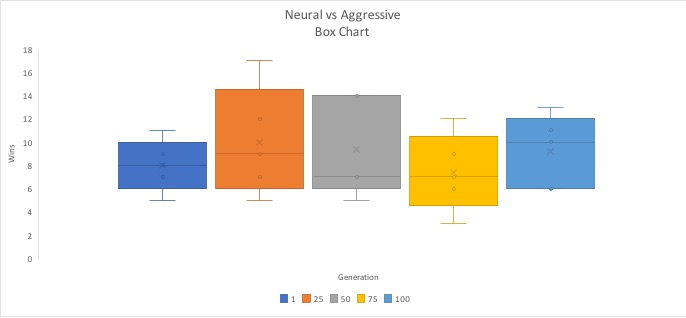
\includegraphics[width = \textwidth]{BoxAgg3.jpg}
	\caption{Box Chart | Neural vs Aggressive | Mutation}
\end{figure}

Overall, neither mating nor mutation present themselves as the more suitable candidate for the primary method of evolution. Both are unfairly offset by the stochastic nature of the game, and are fighting a losing battle.

Across the board, all presented results seem to perform to a mid-range rate of success; Even the hard-coded results are all have a winning score of just above 500 out of 1000. This suggests that regardless of the approach to the game, anyone can and will perform in to an average level.\\

\subsection{External Comparisons}
In a game such as chess with a wide variety of possible moves at any given time, coupled with a knowledge of the opposing players board positions throughout, allows for an intricate neural network setup for evaluating fitness. While it would still present an extremely difficult task to maintain a fair balance with this method, access to the variable values helps quantify the effectiveness of a move.

Contrastingly, Switch is full of unknowns. For example, in chess (assuming a clear understanding of the rules) a player can see potential consequences of making a move before you do it. Meanwhile, in Switch, playing a particular card may make or break a game, with no way of knowing what the potential consequences are without knowing the opponent's hand. 

For example, imagine the neural player has two cards left, and the opposing player is down to their last card. These two cards are the 9 of Hearts, and the 9 of Clubs. The card to be played on top of is the 9 of Diamonds. The neural player then has a decision to make, as both cards are playable. With no idea what the other player holds, the decision cannot be based on anything, and so a card just has to be selected. Now suppose the neural player chooses the 9 of Hearts, and the opponent does not have a Heart, or another 9. This paves the way to victory, as the remaining card can be played. However, if 9 of Clubs had been played instead, it may have allowed the other player to release their final card, which was a club. Similarly, if the opponent had more than one card left in the same scenario, playing the club first may have resulted in the Queen of Clubs being played, forcing the neural player to go from one card to six. Without knowing what other players hold, there is no way to predict the consequence of actions in this way, thus making evaluating the fitness in relation to playing cards would not accurately represent the adequacy of an organism playing the game. 

Thus, without an evaluational function linked to specific cards, it is unlikely to see a case of over-fitting like that on show in the MarI/O simulation where the network learned to continually jump through the level. However, it is not impossible that a card may grow to be favoured over a period of several generations. As previously mentioned, it is possible for an organism to win a single game, and then be killed off for losing immediately after, and so that organism is not going to continue to try to play its favoured card, but due to the fitness being evaluated in a binary fashion in this project, there is a good fair chance that such an organism would be chosen for mating to replace a loser from the population that this one had found success in. As a result of that, it is not impossible for similarities to breed. However, it is safe to assume that any such trend would be minor enough to go undetected. 

\newpage
\section{Critical Evaluation}

\subsection{Achievements vs Objectives}
The initial idea for the project was to build a digital version of the card game Switch, which would be playable by humans, against a neural network. The network would have no indication on what it should do, and how to play the game, with measures in place to ensure that the game did not get stuck, and there were methods of influencing the fitness to promote machine learning in relation to the rules and objective of the game. 

Switch was built and tested in a timely manner to meet the scheduled Christmas target - with the final issue being resolved on Boxing Day in the early hours. The game ran smoothly, had a graphical user interface, and could be played by humans. I was very happy with the project at that stage. 

That happiness was short lived as getting NEAT working turned out to be a real challenge. Without even incorporating any of my own work, WindowsNEAT refused to compile. Having written over 2000 lines of code for my game, I was reluctant to try switching languages, and so I tried to persevere - but to no avail. 

Fortunately I have a Macbook, and was able to get the original version of NEAT to work with that. However, that took far longer than I could have anticipated, as the next section will show. Xcode, the programming environment I used on the Macbook, did not like my code. A lot of alterations had to be made for compatibility reasons, and for a while it seemed like fixing one problem bred two more. Eventually NEAT was bedded in, and I was then able to write my own code to interface the two applications, with some alterations in my own program to accommodate. 

As a result of the switch of operating system, the graphics had to be removed. The library that had been used on Windows does have a Mac version, but enough time was being lost without having to rewrite that as well. Unfortunately this meant losing the functionality of human players too. The code for humans is still in the game, but they are now sadly obsolete. 

This was hugely disappointing as I had hoped to round up my friends from high school against whom I used to play Switch, and ask them to partake in surveys to use as extra results data. 

\newpage
\subsection{Project Management}
At the beginning of the project, a draft timeline was produced. This would always be subject to change, but setting mini-deadlines can help to keep a realistic view of how much time remains for the project.

\begin{figure}[h]
	\centering
	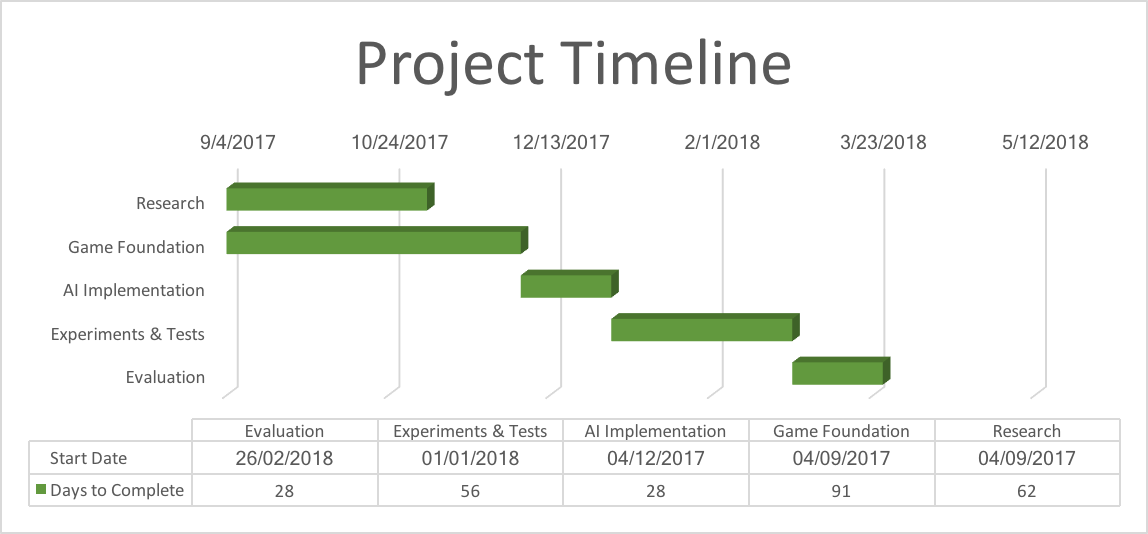
\includegraphics[width = \textwidth]{Gantt1.png}
	\caption{Original Project Timeline Gantt Chart}
\end{figure}

%\begin{figure}[h]
%	\centering
%	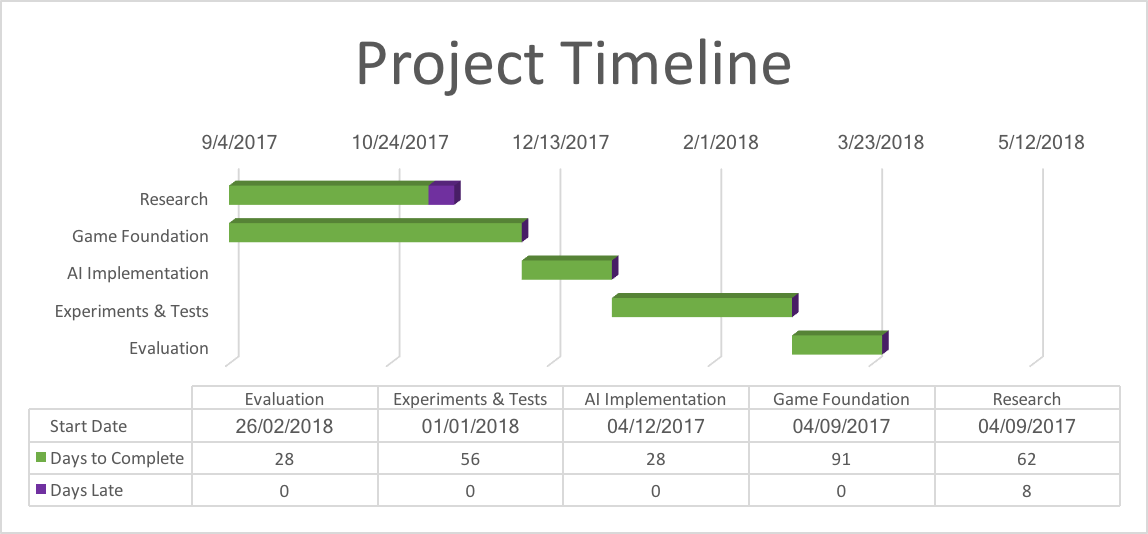
\includegraphics[width = \textwidth]{Gantt2.png}
%	\caption{Updated Gantt Chart - New Year}
%\end{figure}

The research phase of the project ran a little over the initial prediction, but as it ran concurrently with game development, I was able to recover without any early knock-on effects. The foundation of my card game had always been targeted for completion by Christmas - and the final bug was crushed in the small hours of the morning on December 26th. 

%\begin{figure}[h]
%	\centering
%	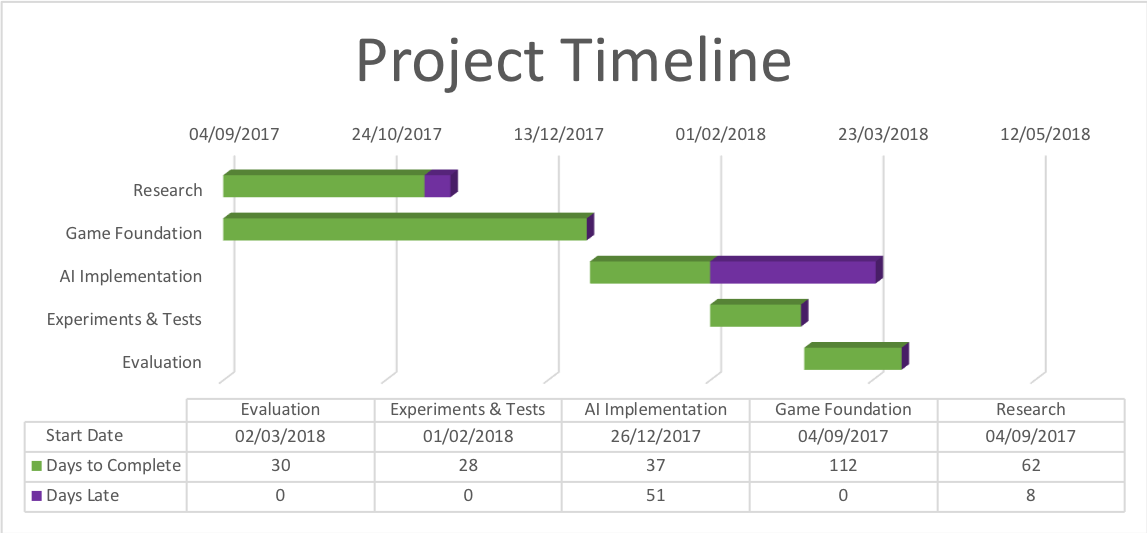
\includegraphics[width = \textwidth]{Gantt3.png}
%	\caption{Post-AI Project Gantt Chart}
%\end{figure}

\begin{figure}[h]
	\centering
	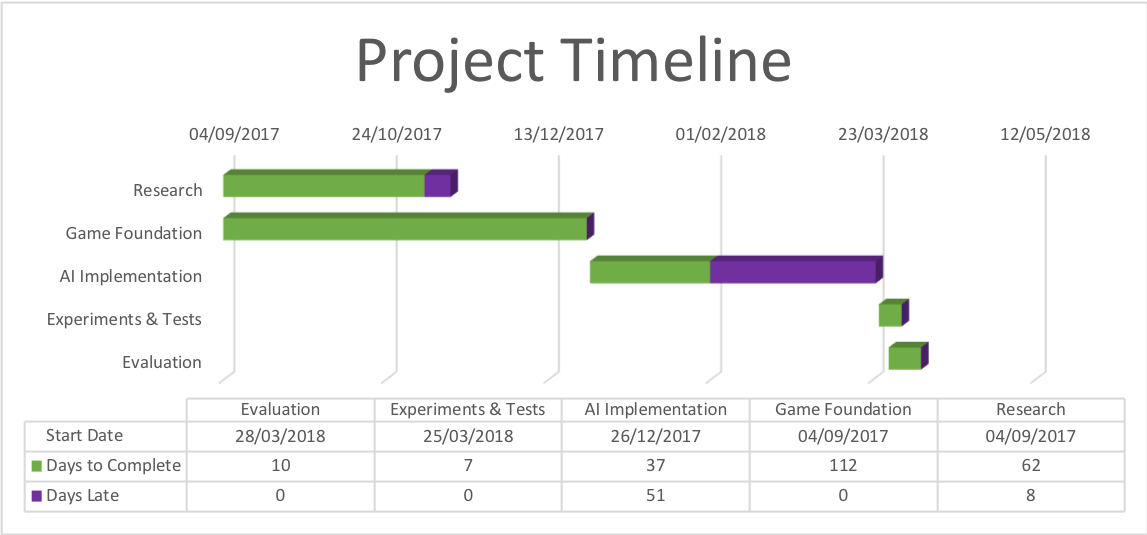
\includegraphics[width = \textwidth]{Gantt4.png}
	\caption{Complete Project Gantt Chart}
\end{figure}

AI implementation took far longer than anticipated due to an unprecedented amount of unforseen issues, and so the final two stages had to be re-evaluated for the final stretch. As a result, these were forced to be completed semi-synergistically.

Despite a much less comfortable closing stage than hoped for, experimentation and evaluation did not suffer to a severe extent.\\

\subsection{Future Work}
I intend to revive the human players by re-introducing SFML, this time with the Mac version. I may also tackle WindowsNEAT again in a bid to make the project accessible on both systems.

It would also be interesting to facilitate multiple neural players with their own networks.\\

\newpage
\section{Conclusion}
Switch is not a game that can be mastered. Players can develop their attitude and methods of play but there is no reliable formula for success, and the hard-coded data proves this. When aggressive and unaggressive play-styles square off, the attacking strategy should theoretically perform extremely well, but the degree at which luck enters the equation means that this is far from the case. No matter how many experiments and generations of tests are carried out, the network is never going to be able to defeat a Switch champion, as such a being does not exist. 

Realistically speaking, the average performance of neural players is akin to that of a human player. Of course, a human that knows the rules well will be able to exercise caution in certain scenarios that the network would not recognise as a potential pitfall, such as choosing to play a Queen of Hearts first when down to two cards and another Heart could have been played first. A human may be aware that they have not seen any black Queens for a while and be wary of allowing one to be played against themselves by selecting their red Queen, whereas the network will not have this kind of information. Or similarly, if all three other Queens have recently been played, playing the Queen of Hearts would guarantee that the opponent has to either pick up or play another Heart, allowing the last card to be played and claim victory. 

Even if allowed to play through every possible permutation of game states repeatedly, it would still be impossible to master the game because there is no way of knowing what the game state is! The only knowledge available is the last card, and the contents of your hand. Thus, it is virtually impossible to truly evaluate effectiveness of the evolution at play throughout the project, as there is no benchmark for what a \textit{good} level entails. 

\newpage
\bibliographystyle{plainnat}
\bibliography{Citations}
%example of References. See https://en.wikibooks.org/wiki/LaTeX/Bibliography_Management
%might be good to use a separate document for these so your main work is not one really long text file. 

%you can crate this on a extra tex document just like the title or any other part of the document.

\newpage
\renewcommand{\thepage}{}
\begin{appendices}
\section{Project Overview}
%insert IPO 

\Large{\textbf{Initial Project Overview}\\

\textbf{SOC10101 Honours Project (40 Credits)}}\\                                                      

\large{\textbf{Title of Project:}}

\normalsize{Evolution of Neural Network Controllers for Gameplay Behaviours} \\

\underline{\textbf{Overview of Project Content and Milestones}}

The idea is to implement a card game with four players. One of the players is the human, another is an AI agent that has no idea how to play the game, and the other two are hard-coded to know the rules and how to play. The intention is for said card game to be Switch, however this is subject to change if the rules are found to be too difficult for the scale of the project – in which case a simpler game will be substituted in.


The agent then learns how to play by trying to make moves based on neural networks. Initially this will be totally random but after the first generation of the algorithm cycle, it will be based on the chromosomes with the highest fitness, which should then begin to provide better results. These moves can be blocked if they are not legal. There will be a scoring system for the agent that will be negatively affected by illegal moves and it will then use this to learn how to do better the next time it plays. The scoring system will also see the agent penalised for losing or not winning. This will be what our fitness is based on. 


It is worth noting that how successful you are in a game of Switch depends entirely on the hand you’re dealt, and how your opponents play the hands they are dealt. A lot of the game is about luck, and so negatively affecting the agent’s score should take this into account and deploy some leniency. 


The project will make use of the NeuroEvolution of Augmenting Topologies (NEAT) library and will most likely be coded in C++. It will use neural network controllers, co-evolving weights and topologies. \\

\pagebreak
\large{\textbf{The Main Deliverable(s):}}
\begin{itemize}
	\item A playable card game that incorporates an Artificial Intelligence agent that must learn how to play the game from scratch based on a score system that penalises the agent for illegal or costly decisions. 
	\item Experimental research into improving the performance (in terms of score) or speeding up the learning process of the agent. 
	\item A report into what positively or negatively affects the agent, and what causes the effects that it has including experiment results using charts and figures. Changes will be made by varying parameter settings of the evolutionary algorithm in a systematic way.
\end{itemize}

\large{\textbf{The Target Audience for the Deliverable(s):}}

Whilst the final product will be a playable game, it will really be aimed more at being experimental research into Artificial Intelligence techniques and, more specifically, evolving neural network controllers for playing games. Thus, the audience most likely to be interested in the project are those who also want to look into artificial intelligence agents. \\

\pagebreak
\large{\textbf{The Work to be Undertaken:}}
\begin{itemize}
	\item Design and build a game of Switch without the AI agent
	\item Thoroughly test the bare-bones game to ensure it works perfectly without bugs
	\item Research neural networks and evolutionary algorithms
	\item Implement the AI agent
	\item Experiment with a few different techniques and test how they perform in terms of improving or decreasing the agent’s intelligence/performance in game.
\end{itemize} 

\large{\textbf{Additional Information / Knowledge Required:}}

Neural networks and evolutionary algorithms\\

\large{\textbf{Information Sources that Provide a Context for the Project:}} %HATE how Project is on the next line here
\begin{itemize}
	\item Lubberts, \& Miikkulainen (2001). Co-Evolving a Go-Playing Neural Network.
	\item Stanley, Bryant, \& Miikkulainen (2005). Evolving Neural Network Agents in the NERO Video Game. IEEE Press.
	\item Thrun (1995). Learning to Play the Game of Chess. MIT Press. 
\end{itemize}

\large{\textbf{The Importance of the Project:}}

Exploring possibilities and limits of AI in games, particularly evolved controllers which do not have to be hard-coded.\\

\large{\textbf{The Key Challenge(s) to be Overcome:}}
\begin{itemize}
	\item Complete lack of knowledge and experience with Artificial Intelligence techniques
\end{itemize}

\newpage
\section{Second Formal Review Output}
%Insert a copy of the project review form you were given at the end of the review by the second marker

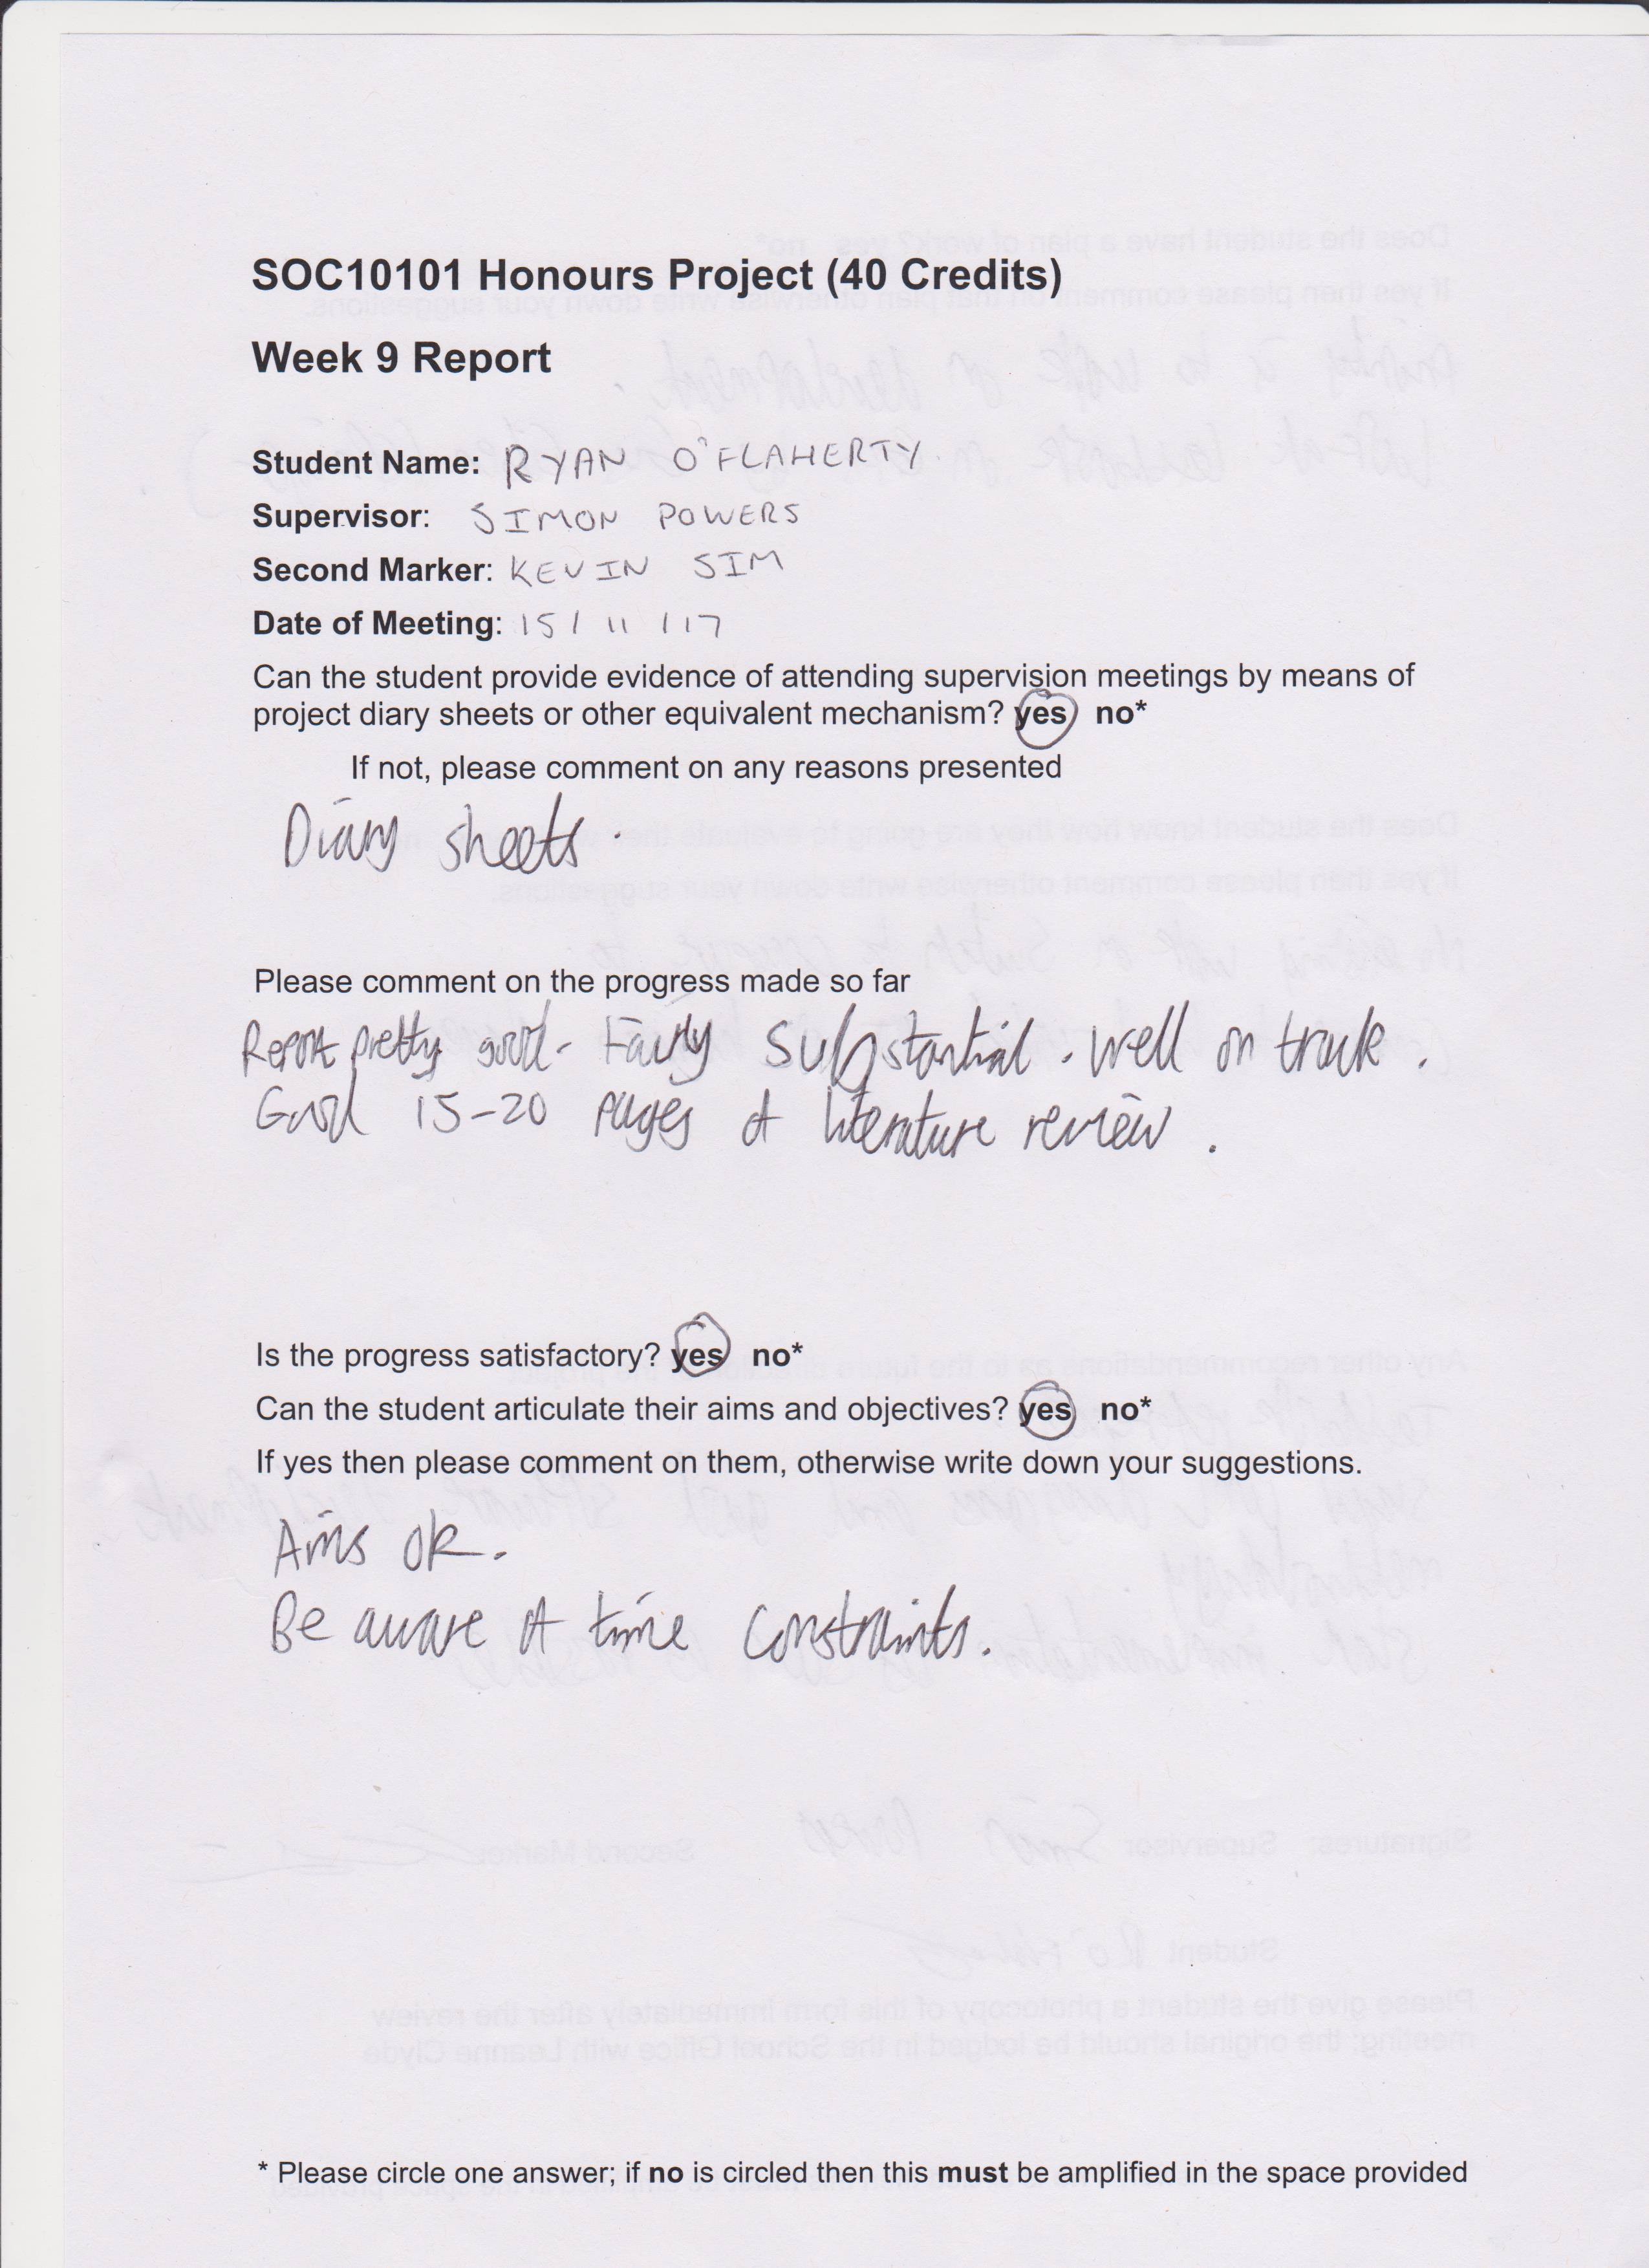
\includegraphics[width=\textwidth]{Week9Report1.jpg}

\newpage
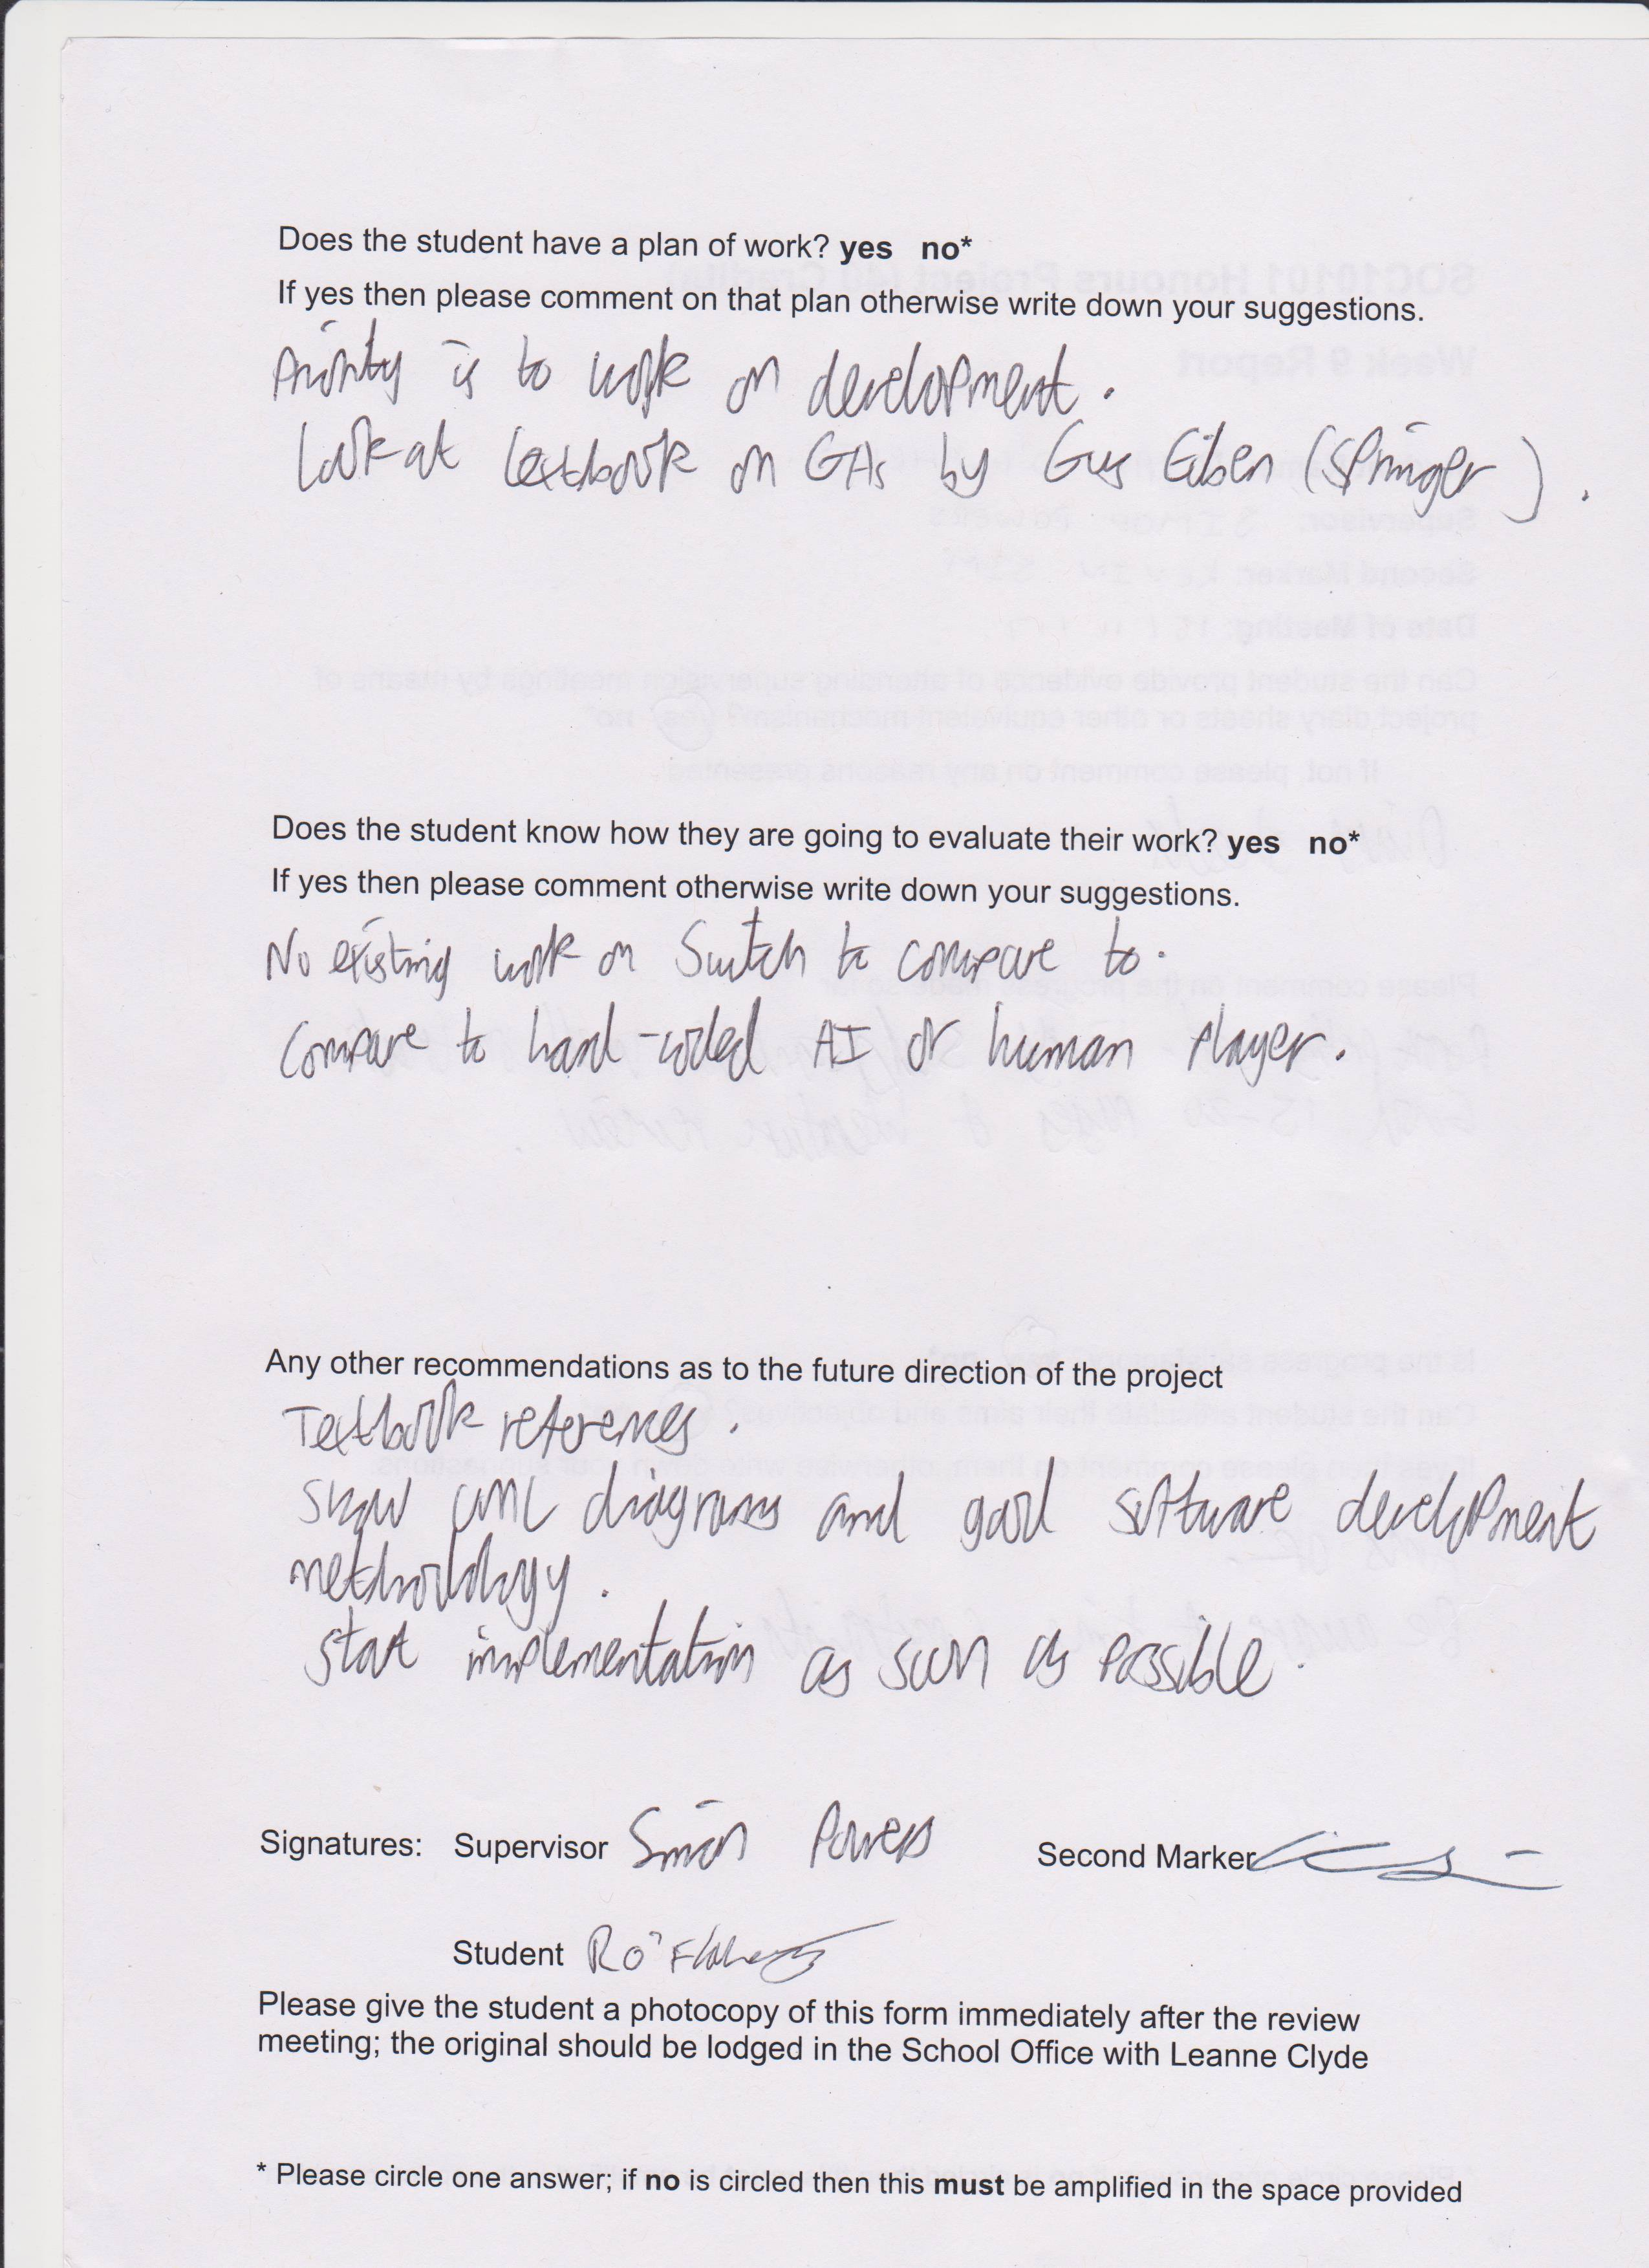
\includegraphics[width=\textwidth, height=\textheight]{Week9Report2.jpg}

\newpage
\section{Diary Sheets}
%(or other project management evidence)
%Insert diary sheets here together with any project management plan you have

%Includepdf starts on a new page which is kinda a pain
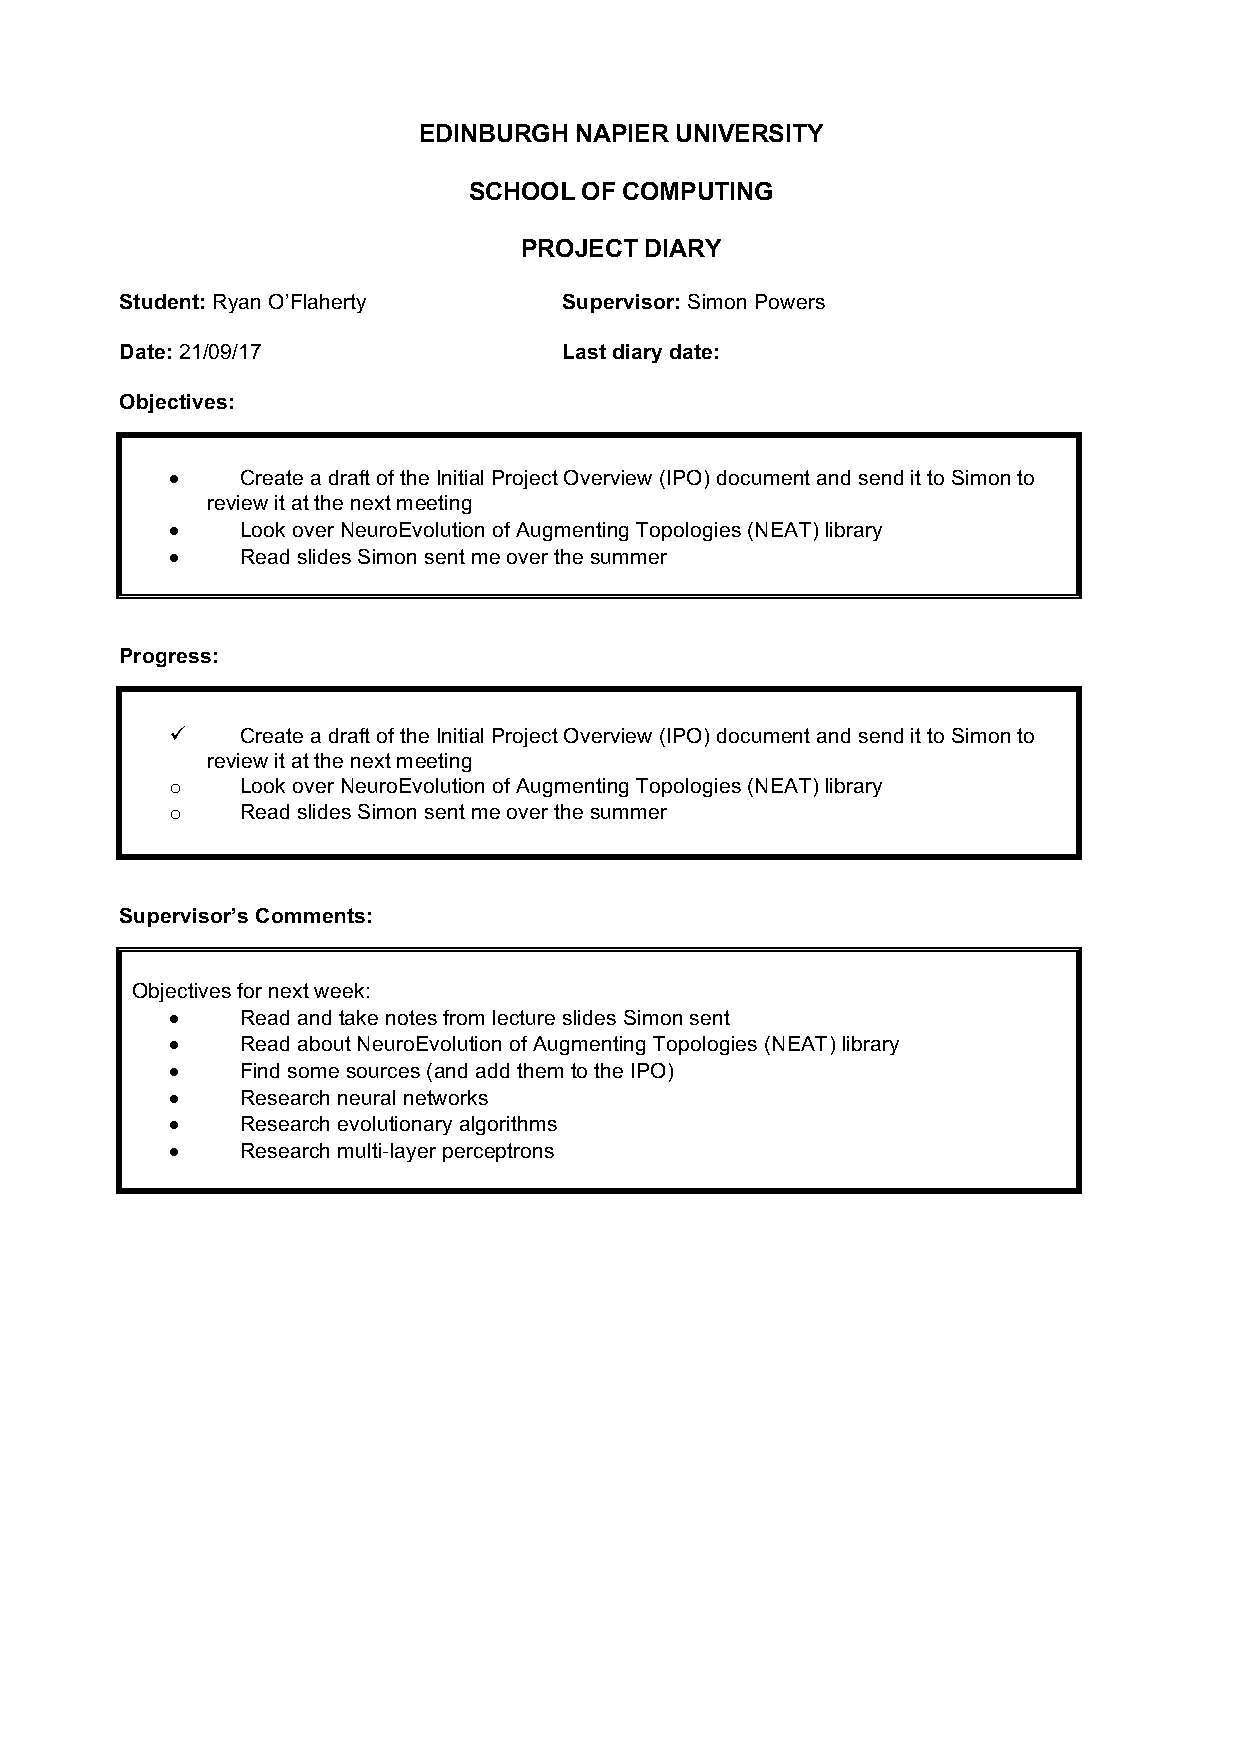
\includepdf[ pages=-,pagecommand={},width=\textwidth]{SupervisorMeetings/All.pdf}

\newpage
\section{Timeline Gantt Charts}

\begin{center}
	{
		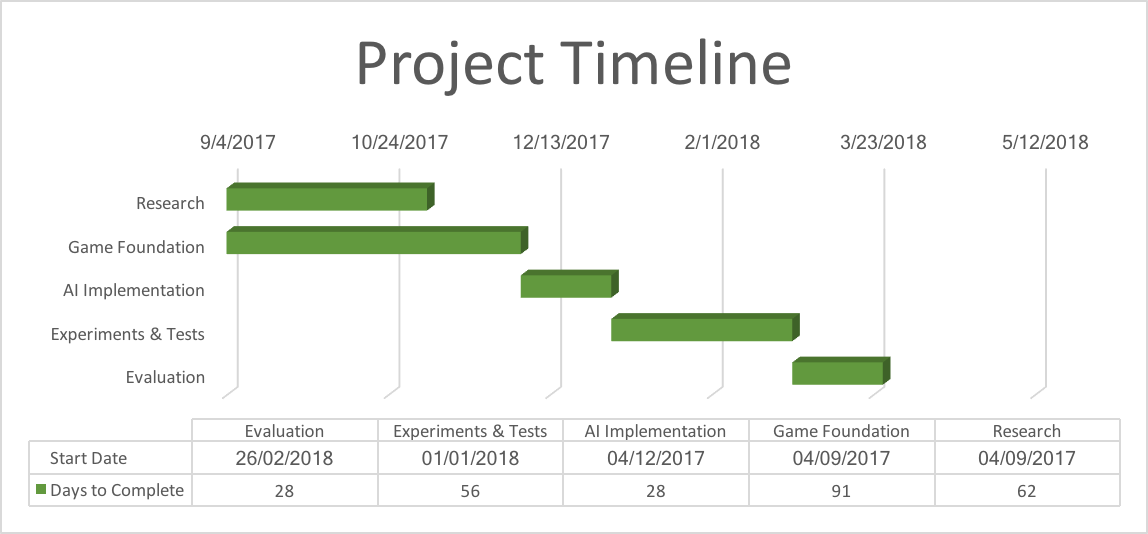
\includegraphics[scale = 0.5]{Gantt1.png}
		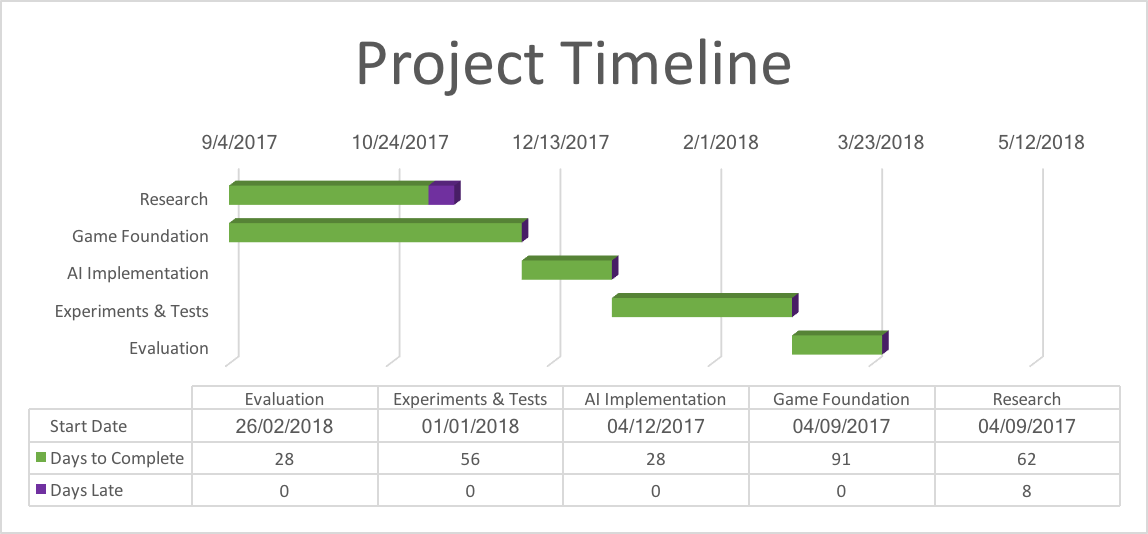
\includegraphics[scale = 0.5]{Gantt2.png}
		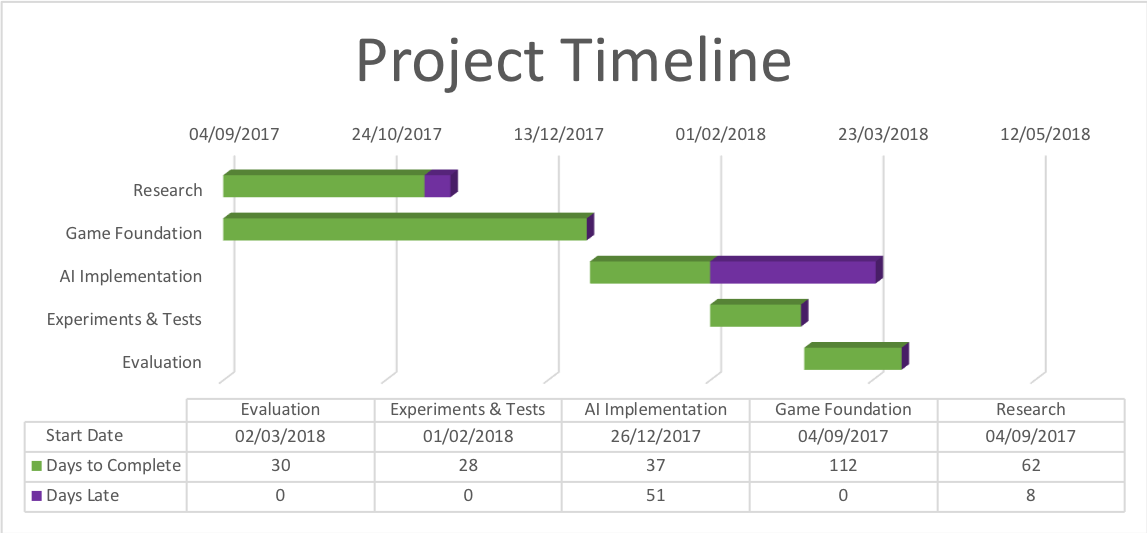
\includegraphics[scale = 0.5]{Gantt3.png}
		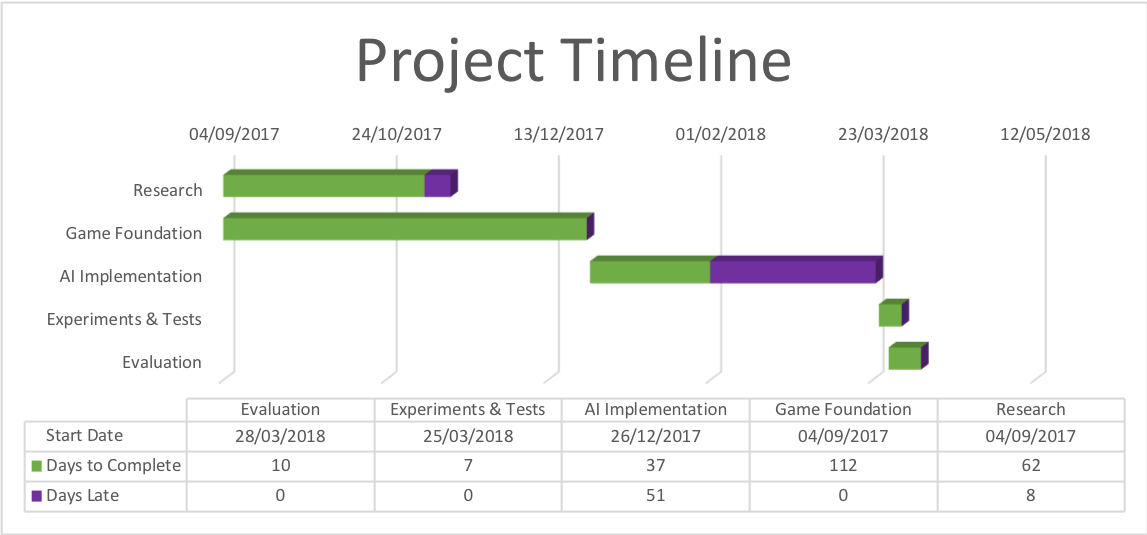
\includegraphics[scale = 0.5]{Gantt4.png}
	}
\end{center}
	

\newpage
\section{My Website}
\href{http://www.x4iiiis.com/honoursproject}
{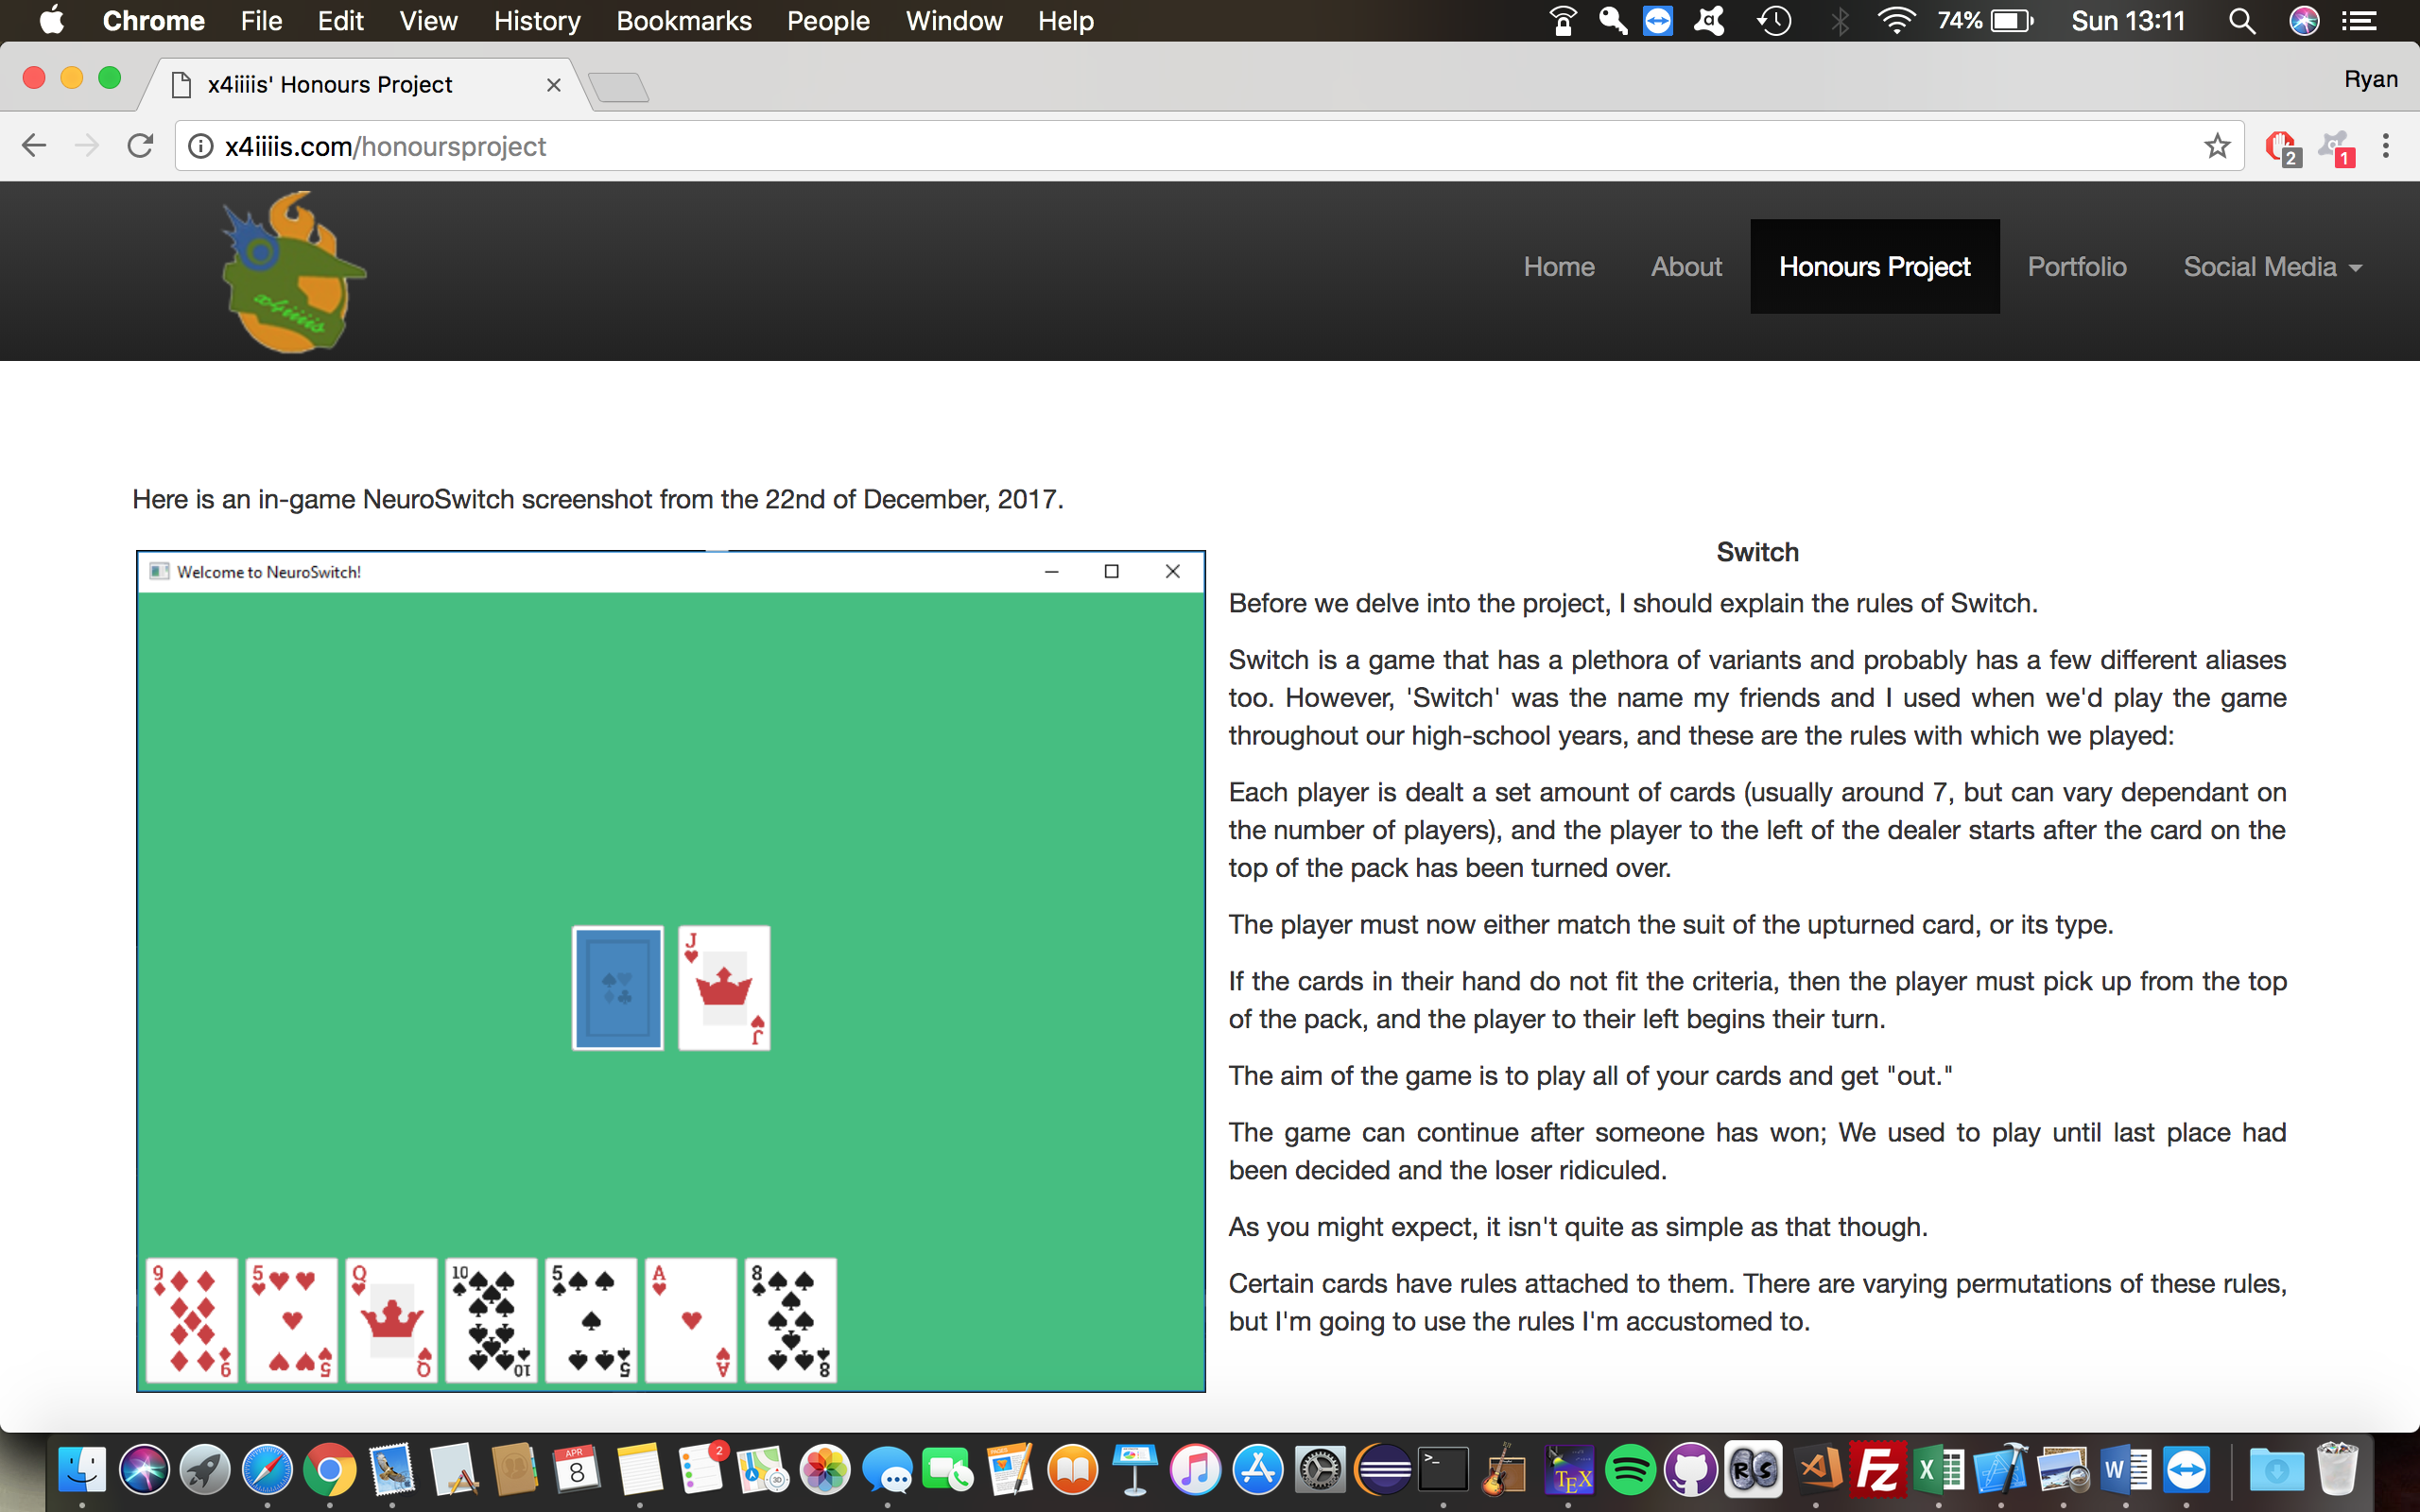
\includegraphics[width=\textwidth]{Website.png}}

\begin{center}
	{\href{http://www.x4iiiis.com/honoursproject}{www.x4iiiis.com/honoursproject}}
\end{center}


\newpage
\section{Textures}
\href{https://opengameart.org/content/boardgame-pack}
{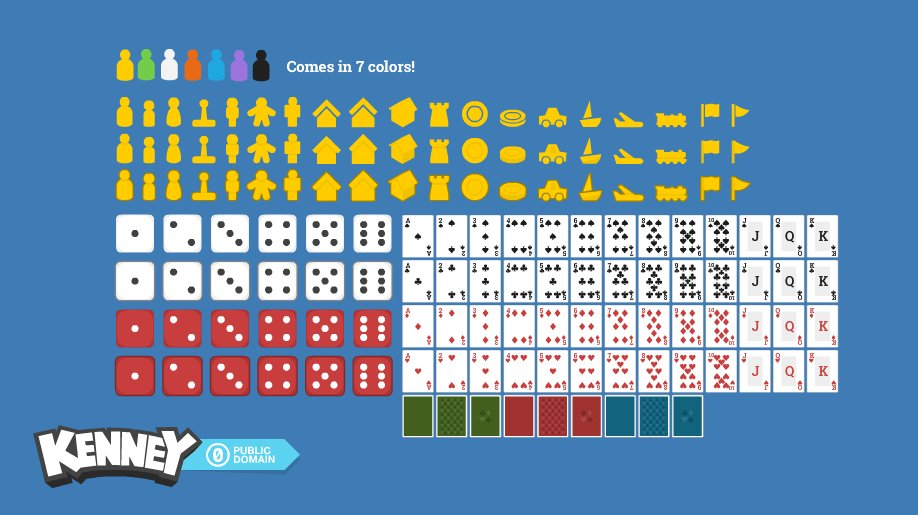
\includegraphics[width=\textwidth]{Kenney.jpg}}

\begin{center}
	{\href{https://opengameart.org/content/boardgame-pack}{www.opengameart.org/content/boardgame-pack}}
\end{center}


Playing card textures used in NeuroSwitch were courtesy of Kenney Vleugels, coming as part of his boardgame texture pack.\\

\newpage
\section{NEAT Documentation/Tutorial}
The documentation file used throughout the use of the NEAT library is found as part of a download at the link below. The file is called NEATDOC.ps.

\begin{center}
\href{http://www.cs.utexas.edu/users/nn/downloads/software/neat.1.1.tar.gz}{http://nn.cs.utexas.edu/soft-view.php?SoftID=4}
\end{center}

Alternatively it can be viewed as a Portable File Format at

\begin{center}
	\href{http://x4iiiis.com/honours/NEATDOC.pdf}{www.x4iiiis.com/honours/NEATDOC.pdf}
\end{center}

%\newpage
%\section{Appendix 7 and following}
%insert content here and for each of the other appendices, the title may be just on a page by itself, the pages of the appendices are not numbered, unless an included document such as a user manual or design document is itself pager numbered.

\end{appendices}

\end{document}
